\documentclass[12pt,a4paper]{article}

% Enable hyperlinking for references and indexes

\usepackage{hyperref}

% Code styles and colours

\usepackage{listings}
\usepackage{xcolor}

\definecolor{codegreen}{rgb}{0,0.6,0}
\definecolor{codegray}{rgb}{0.5,0.5,0.5}
\definecolor{codepurple}{rgb}{0.58,0,0.82}
\definecolor{backcolour}{rgb}{0.95,0.95,0.92}

\lstdefinestyle{mystyle}{
    backgroundcolor=\color{backcolour},
    commentstyle=\color{codegreen},
    keywordstyle=\color{magenta},
    numberstyle=\tiny\color{codegray},
    stringstyle=\color{codepurple},
    basicstyle=\ttfamily\footnotesize,
    breakatwhitespace=false,
    breaklines=true,
    captionpos=b,
    keepspaces=true,
    numbers=left,
    numbersep=5pt,
    showspaces=false,
    showstringspaces=false,
    showtabs=false,
    tabsize=2
}

\lstset{language=Python}
\lstset{frame=single}
\lstset{style=mystyle}

% Figures configuration

\usepackage{graphicx}
\usepackage{float} %to use the option "H"

\graphicspath{ {./images/} }


% \usepackage[none]{hyphenat}

\begin{document}

\title{Beyond Metadata for BBC iPlayer:\\an autoencoder-driven approach for embeddings generation in content similarity recommendation}
\author{Simone Spaccarotella}
\date{4th November 2024}

\pagenumbering{roman}

\maketitle
\thispagestyle{empty}
\newpage

\tableofcontents
\lstlistoflistings
\listoffigures

% Explain who you are, what your role is and why this project is relevant to yourself, remember the assessor will not have met you before.
% Give some context with relevant information on the organisation.

\section{Introduction and background}

I am a Software Engineer at the BBC, Team Lead for the Sounds web team, and I have been training as a Data Scientist,
working in attachment with the iPlayer Recommendation team.

I built a machine learning model pipeline that generates content-to-content (C2C) similarity recommendations
of video on-demand (VOD), for the ``More Like This'' section on BBC iPlayer \cite{BBC:MoreLikeBluey}.
This project is relevant to me because I have been crossing paths with the world of recommendations
multiple times during my career at the BBC, and it sparked an interest.
I had a tangent encounter back in 2015 while working for a team that was building
an initial recommender for BBC News, and an API to provide recommendations using 3rd party engines.
During a Hack Day sometime later, I produced and presented a talk called
``Recommendation Assumptions'' \cite{RecsAssumptions}, which was about types of recommendations and external factors affecting
them, which are contextual to the consumption of the content itself. Until these days, where I was able to finally put my knowledge into practice
with an actual project on real data.

The BBC is a well-known British broadcaster, and it is always evolving to remain relevant to its audience. Its mission
is to inform, educate and entertain, and it operates within the boundaries set by the Royal Charter \cite{BBC:RoyalCharter}.
The current media landscape requires the BBC to deliver digital-first content that is relevant to the audience,
and this involves investments in data and personalised services, not to mention a certain revolution in
generative machine learning modelling that is keeping everyone busy.


% Give a brief overview of what the project is and what the intended outcomes are.
% Emphasise the potential benefits of the project with quantifiable information.
% We should frame this as a problem to be solved

\section{Outline of the issue or opportunity and the business problem to be solved}

The BBC produces and stores a vast amount of data for its content, and this data is produced and surfaced by countless services and APIs.
One of the priority for the BBC is to increae the usage across the business of "Passport" tags \cite{BBC:PassportMetadata} an internal BBC
system that provides a richer set of metadata annotations for multi modal content (audio, video and text).
The usage in production is very low, and its BBC-wide adoption would make the access to metadata consistent,
removing duplications and reducing effort and costs.

Furthermore, the similarity score of the current C2C recommender is directly proportional to the number of values in common between any pairs of items
on a per-feature basis. But the commonality is calculated with an exact string equality, hence it ignores any relationship between different
categorical values expressing a similar concept (e.g. "comedy", "stand-up comedy").

Moreover, the number and types of tags are not enough to sufficiently
describe the content, while the data distribution is severely skewed towards the most popular annotations and no pre-processing
is applied.

Lastly, each similarity score is multiplied by a hardcoded weight that modulates the importance of a feature, but it doesn't solve
the polarising effect of a skewed distribution. Unfortunately, because they are hyperparameters and not learned weights, the model can't improve
its performances by minimising them against a cost function.
\\ \\
To address these issues, the aim of this project was:

\begin{itemize}
  \item \textbf{To improve the quality of the C2C similarity recommendations}. The hypothesis was that by using in input a richer set of metadata that
  better describes the content, and by reducing the high-dimensional data to a lower-dimensional latent manifold,
  the model would be able to generate embeddings that could improve the quality of the recommendations, by mapping the
  item similarity problem to a geometric distance calculation between vectors in a multi-dimensional Euclidean space.
  \item \textbf{To reduce the costs to generate C2C similarity recommendations}. I used Passport tags as input to build a general solution
  that could be used by any product and applied to any type of content, because they all share the same set of common annotations.
  \item \textbf{To build a foundational item-embeddings generator}. Content-based recommenders
  use item metadata. This project provided an immediate solution for C2C unpersonalised recommendations that solely relies on them and
  it could provide a foundational approach for personalised recommender that combine content metadata with other signals like user interactions
  and contextual data.
\end{itemize}


% Provide high-level overview of the methods (e.g. regression) and tools used
% with justification explaining why these methods are suitable for the problem at hand.
% Justification may include factors such as the need for interpretability, transparency
% or the timescales you had to work with.

\section{Methods and justification}

\subsection{Data pre-processing}

I used \textbf{one-hot encoding} to transform the categorical features (i.e. the metadata annotations) into a numerical vector.
It's a simple yet effective encoding method and it's perfect for the transformation of nominal categoricals,
because it doesn't introduce any ranking and/or arithmetic relationship among the
encoded values. The downside of this approach is that it generates high-dimensional sparse arrays,
introducing the so-called \textit{curse of dimensionality} problem. Nonetheless, this was an accepted drawback that was
managed in the modelling phase.

\subsection{Modelling and regularisation}

I trained an \textbf{autoencoder} \cite{DBLP:journals/corr/abs-2003-05991,DBLP:journals/corr/abs-2201-03898}
to learn latent features of the Passport tags, and to reduce the size of the encoded vectors.
The autoencoder is a type of encoder-decoder neural network, a self-supervised model capable of capturing non-linearity from the data.
I used the ``undercomplete'' variant, that constrains the number of nodes in the hidden layers, creating a ``bottleneck''
of information flow through the network.
This bottleneck is a form of \textit{regularisation} that forces the model to learn latent attributes from the input,
while reconstructing it with minimal loss. Ultimately, it prevents the model from \textit{overfitting} the training dataset,
by indexing it like a caching layer.

The trained \textit{encoder} segment of the network, was used to compress the one-hot encoded high-dimensional sparse array into
a lower-dimensional and denser representation called \textit{embedding} \cite{GoogleForDevelopers:Embeddings}.
This technique solved the curse of dimensionality and the data sparsity problems, and improved the calculation complexity and the quality
of the recommendations at inference time.

To improve and assess the ability of the model to \textit{generalise} on unseen data, I randomly shuffled the dataset and split
it into 3 chunks: training, validation and test. I run \textbf{hyperparameter tuning} to find the best set of model parameters
that minimised the objective function and I used the validation set to regularise the model with \textbf{early stopping}.
This technique monitored the reconstruction loss on an out-of-sample dataset,
allowing the model to stop training within a set ``patience'' threshold, after reaching a local minimum on the validation error.

I used \textbf{dropout} to further regularise the model and make it robust to small changes in the input,
and \textbf{data augmentation}, by including in the training data the episodes of a programme that share the same tags with their
parent container.

\textbf{Weight decay} and \textbf{batch normalisation} were tested during hyperparameter tuning and discarded for poor performances.

\subsection{Inference}

Item similarity was calculated with the \textbf{cosine} of the angle $\theta$ between each pair of embeddings \cite{GoogleForDevelopers:EmbeddingSimilarity}.
This metric is insensitive to the magnitude of the vectors, and because high-frequency values tend to have a larger magnitude, it mitigates the impact of
popularity in the similarity calculation. One-hot encoded vectors lack of meaningful relations between them.
They represent unit vectors bound in the ``positive quadrant'' of a Cartesian coordinate system for a multi-dimensional Euclidean space.
Because each pair can only have a finite number of angles,
the cosine similarity will also assume a finite number of discrete values between 0 and 1, causing information
loss. Ideally, we would expect the similarity score to assume a continuous value bound between -1 and 1, and this
is only possible if the angle $\theta$ of any vector pair can assume a continuous value between 0 and 360 (i.e. $0\pi$ and $2\pi$), hence
the use of embeddings.

\subsection{Tools and frameworks}

The entire project was written in \textbf{Python}. It is the \textit{de facto} programming language for data science
and machine learning tasks. Python has an established, diverse and well-documented ecosystem of external libraries
and frameworks that facilitated the job, and it is also the language of choice at the BBC.

I used \textbf{Pandas} only for tabular data manipulation, to generate and store the one-hot encoded vectors. Unfortunately, it wasn't possible
to use it for exploratory data analysis (EDA), because the iPlayer catalogue used in development had roughly one-year worth of data and it didn't
fit in memory, causing Pandas to crash. For this reason, I used \textbf{Dask}. It is a library capable of running out-of-memory and
parallel execution for faster processing on single-node machines and distributed computing on multi-nodes machines, while using the familiar Pandas API.

I used \textbf{TensorFlow} and \textbf{Keras} for modelling, to build and train the encoder-decoder neural network architecture,
and \textbf{Keras Tuner} for
hyperparameters tuning. I also used \textbf{Scikit-learn} but not for modelling. It provided utility functions for the dataset splitting and
the cosine similarity calculation, and I was already familiar with its API.

For data visualisation I used a combination of \textbf{Matplotlib} and \textbf{Seaborn}, while I used \textbf{rdflib} to fetch and parse
the RDF documents from the BBC Ontology. These documents represented the metadata values and contained the actual entity label.
This label was needed to hydrate the set of metadata for each item, to visualise the recommendations for testing purposes.
Worth also mentioning the use of \textbf{pytest} for unit testing and \textbf{black} for PEP 8 code compliance and formatting.
Finally, I used \textbf{Jupyter Lab} to edit the project, \textbf{git} for code versioning, \textbf{GitHub} as a remote code repository
and for collaboration, and \textbf{AWS Sagemaker} to run the pipeline on more capable virtual machines, especially during hyperparameter tuning.


% Detail what the minimum desirable outcome is and how success will be measured.

\section{Scope of the project and Key Performance Indicators}

The minimum desirable outcome for this project was to build an end-to-end machine learning solution able to produce content-to-content
similarity recommendations using Passport metadata tags as input. On a qualitative level, success meant producing recommendations
comparable with the ones currently in production. This was initially tested by visualising and manually comparing the similarities and differences
of the two result sets. A panel of stakeholders with diverse domain knowledge was involved to give their subjective feedback.

The usage of Passport tags was a success/failure boolean measure, while the coverage and spread of the metadata among the
top K recommended items with respect to the seed item was used as a quantitative measure of diversity.


% This gives a good opportunity to briefly describe the data architecture of your company
% You must show you have considered all relevant data protection policies and regulations (both internal company policy and external laws or guidelines).
% If you use any data external to the company you must reference it.
% Justify the choice of the data and why it is relevant to the project
% State what tools you used to efficiently gather the data
% Outline briefly the data cleansing steps you have taken and the consideration of any source of error and bias
% Survey of potential alternatives
% Best practice in any data science problem is to consider a range of appropriate models
% Detail the alternative models
% State the pros and cons of each, including the justification for your chosen approach.
% Critical evaluation of your methods is key
% Implementation - performance metrics
% The efficacy of your chosen model will be one of the main factors behind choosing it as your approach and dismissing alternatives.
% This can be demonstrated by showing a range of performance metrics for the model you have chosen as well as for the alternatives considered
% Justify your choice of metrics stating why they are appropriate for this particular implementation of machine learning
% It may be easiest to present these metrics and methods in a tabular format

\subsection{Data selection, collection \& pre-processing}

News articles, iPlayer videos on-demand, etc. are annotated with the so-called Passport tags.
These tags describe the content, and the annotations are either applied manually
by an editorial team with domain knowledge, or semi-automatically by machine learning algorithms with human supervision.

Passport tags are distributed via the universal content exposure and delivery (UCED) system,
a self-service metadata delivery platform that exposes data as a document stream for product to integrate with.
This platform provides different types of "consumers" such as REST API, AWS S3 bucket, etc.
Passport documents are JSON objects that contain a property called "taggings", an array of objects representing the
metadata annotations. These objects in turn contain two properties: "predicate" and "value". They represent the name and the value of
a tag, and are expressed as URL-formatted strings. The predicate refers to a class of the BBC Ontology \cite{BBC:Ontologies}
and the value to an entity stored as an RDF document, accessible in Turtle format \cite{W3C:Turtle} via the BBC Things API \cite{BBC:Things,BBC:Things:About,BBC:Things:API}.

For the development of the project, I decided not to integrate with UCED but to use batches of Passport files, manually collected and stored
on a local folder.
This was a tradeoff that allowed me to develop the project with real data while keeping the costs down, given that the resources needed to
be set on two AWS accounts. Moreover, I didn't want to pass the burden of maintenance to the team the owned the accounts, without having tested
the feasibility of the solution first.

Content metadata is not classified as personally identifiable information (PII), according to the UK GDPR \cite{UKGDPR}. Nonetheless,
this data is regulated by the internal BBC data governance and it is encrypted at rest and in transit. For this reason, no other precaution
were required during storage and processing.

I chose to use Passport because this data provides a flexible and shared set of tags that can annotate any type of content produced by the BBC,
making this a general solution that reduces duplications and ultimately costs. Passport provides a rich set of tags to describe
the content. For example, an iPlayer programme can be described not only in terms of the canonical genre or format. Annotations can describe
the "contributor" that features in it, the "narrative theme", what this programme is "about" or what relevant "entities" are mentioned in it
and many more.

% Outline briefly the data cleansing steps you have taken and the consideration of any source of error and bias
% Survey of potential alternatives
% Best practice in any data science problem is to consider a range of appropriate models
% Detail the alternative models
% State the pros and cons of each, including the justification for your chosen approach.
% Critical evaluation of your methods is key
% Implementation - performance metrics
% The efficacy of your chosen model will be one of the main factors behind choosing it as your approach and dismissing alternatives.
% This can be demonstrated by showing a range of performance metrics for the model you have chosen as well as for the alternatives considered
% Justify your choice of metrics stating why they are appropriate for this particular implementation of machine learning
% It may be easiest to present these metrics and methods in a tabular format
The tags are entities linked to each other or to external resources and are described by attributes and relationships defined by the BBC Ontology,
according to the RDF \cite{W3C:RDF,W3C:RDF:Concepts} standard.
This makes the dataset a graph. I initially considered using a Graph Neural Network to exploits these relationship,
but this would have inflated the complexity of the project, increasing the risk of not finishing it on time.

During pre-processing, a list of JSON files were loaded into the pipeline and the tags extrapolated into a dictionary data structure, where the key represented
the programme ID (called PID) and the value an object of predicate/value Passport tags. A programme can be tagged with the same predicate multiple times,
as long as is done with different values, while the same value (e.g. "Music") can be used by multiple predicates (e.g. "about" or "genre").

The dictionary was transformed in a Pandas Dataframe, where the rows represented the programmes and the columns the tags.
I used a MultiIndex \cite{Pandas:MultiIndex} for the columns because of the duplicate values across predicates.
I then populated the cells with "1" if the programme was tagged with the corresponding tag, with "0" otherwise, generating a
list of multi-hot encoded arrays.

Selection bias was a possibility during the data collection phase. A programme with an empty list of tags could have been due to
an actual absence of them, or because I missed the while searching for the input batches. To mitigate this, I retrieved a list
of all available programmes on the iPlayer catalogue during a given timeframe, and searched for the related tags.
If the file wasn't available, it meant no tags were generated.


% Best practice in any data science problem is to consider a range of appropriate models
% Detail the alternative models
% State the pros and cons of each, including the justification for your chosen approach.
% Critical evaluation of your methods is key

\section{Survey of potential alternatives}

Given a numerical vector representing the Passport tags of a programme in input, the model needed to return a list of the top-k programmes,
sorted in a descending similarity order.
The geometric interpretation of the similarity between two items, is the distance between the two vectors representing them.

I considered using a Clustering technique to group "similar" items together, so that given an item in input, the model would return
the ones belonging to the same cluster. I didn't know how many cluster there were in the data, and I didn't need to know.
I could have used a density-based technique to autodiscover them,
but even in that case, some of the clusters could have had less than K items in a top-K similarity scenario.
I could have returned the items belonging to the nearest cluster if needed, but at that point,
what's was the meaning of clusters in that context anyway?
In content similarity, any item has a degree of similarity with
all the others and clustering was just a coarse-grained discretisation of that concept.
I needed a more granular approach where every item could be compared with anyone else.
In geometric terms it meant that I had to calculate the pairwise distance between any two pairs of vectors, so I didn't need to use
clustering in the first place.

Both clustering and pairwise distance use the concept of gemoterical distance between any two pairs, and this calculation
is computationally expensive, and doesn't scale on big datasets, especially if it involves high-dimensional sparse arrays.
Not only that, the one-hot encoding processing doesn't use any spatial proximity information to transform the categorical features
into ones and zeros. It's a plain transformation that pivots the unique values of a given variable as features, and sets 1 to the
corresponding annotations. If we take this raw vector as is, and interpret it as a multi-dimensional coordinate system and then calculate
similarity, we are out of luck.

From a computational point of view, I needed to handle the curse of dimensionality, by reducing the dimension of the numerical vectors.
Not only that, the new vectors needed to be in a denser and lower dimensional manifold embedded into the original high-dimensional ambient space,
for the "local proximity" to have a meaning in terms of similarity.

Dimensionality reduction techniques such as Principal Component Analysis (PCA) (which I'm more familiar with), or
Independent Component Analysis (ICA), Linear Discriminant Analysis (LDA), etc. were next on the list, but there was a problem with them too.
Their job is to find a linear projection of the data and this is a strong assumption that - more ofthen than not - misses important non-linear
structures in the data. So, I discarded the idea of using PCA, but not the idea of using dimensionality reduction.
I just needed a non-linear aproach, so I turned my attantion to manifold learning.

Before discussing that, I'd like to point out that I also considered changing the pre-processing step to generate a different
set of vectors that didn't suffer from the curse of dimensionality.

Hashing is a well-known non-invertible technique that can be used in machine learning for feature reduction.
The reason why I didn't adopt this technique was because hashing has more hyperparameters than one-hot encoding, which increase its complexity.
Settings like the size of the hash could have impacted the descriptive power of the vector even before starting the embedding learning phase.
But most importantly, hashing functions introduce the collision problem, were two distinct entities can be mapped to the same index in the target domain.
Because this is an issue that can't be removed, only mitigated, I tested the latest and strongest algorithm to reduce the likelihood of collisions,
but the trade-off was too computetionally expensive during training.

I talked about why I adopted one-hot encoding, let's now talk about my chosen approach for manifold learning, pros and cons and its justification.


% Implementation - performance metrics
% The efficacy of your chosen model will be one of the main factors behind choosing it as your approach and dismissing alternatives.
% This can be demonstrated by showing a range of performance metrics for the model you have chosen as well as for the alternatives considered
% Justify your choice of metrics stating why they are appropriate for this particular implementation of machine learning
% It may be easiest to present these metrics and methods in a tabular format

\section{Implementation and performance metrics}


\section{Discussion and conclusions}

% These should be framed as benefits to the business with quantifiable evidence
% It is likely the results of your project will have been shared at the company,
% if they were shown in a presentation or perhaps in a dashboard state this. If positive feedback was received, include this also.
% Reconsider your stakeholders, did the project have the expected outcomes for them?
\subsection{Results}

This is a general solution that works on any content that uses Passport tags. It could be implemented as a single implementation
to serve multiple products. This will reduce effort, duplication of code and data, and as a consequence, costs.
I presented this project explaining the main intuition and showing the results with the visualisation tool.
Once to the data scientists and engineers of the team I worked with and on a second occasion,
to the stakeholders of the team that - after an internal restructuring - will be in charge to provide non-personalised recommendations,
including C2C similarity. The feedback was positive in both cases. When I presented the project to the last team, it was mentioned
that we would need to implement this solution so that we can assess end-to-end feasibility and put it in a position to be A/B tested
against the current solution in production.

% State how your results have aligned with your original objectives and measures of success
% State what recommendations have been made to the business as a result of this project
% These recommendations may include proposals for further work or alternative research or extensions to the project
% State whether or not the machine learning approach can be successful in meeting the future requirements of the business.
% If it has been deployed state considerations such as data drift and retraining that will need to be taken into account
% It has not been deployed but there is a desire to do so within the business outline and the steps needed to achieve this
\subsection{Summary of findings and recommendations}

The results are perfectly aligned with the initial objectives and measure of success set at the beginning of the project.
My recommendation is to build an initial minimum viable product (MVP) pipeline on the AWS development account.
This will allow us to break down the engineering effort, and to spot any blockers/challenges that need to be addressed
as early as possible, so that we can correct them and/or reconsider some of the assumptions ahead of the production build.
We could use the Sagemaker Pipeline to build the stages, and initially test the end-to-end solution with batch Passport data.
We would need two pipelines, one for training and one for inference, to generate the embeddings and the similarity scores.
The output could be cached, to improve performances, and if everything goes smoothly from an engineering point of view,
we could integrate with UCED to fetch real-time data, and prep the solution for A/B testing.

If this solution is viable and passes the A/B test, it could also be used to generate embeddings for
other personalised recommenders that use item metadata in conjunction with user interactions and/or contextual data such as
day and time of interaction, location, device used, etc.

The project could be further expanded by exploiting the graph nature of the data using graph neural network (GNN), specifically a
graph autoencoder (GAE) to learn meaningful representation of the graph data, capturing the topological structure and the node content.
This could improve upon the current autoencoder, that relies on the same data being flattened.
This effort will require further research and prototyping.

% Outline the repercussions the execution of this project has had for yourself, your colleagues, the stakeholders and the business as a whole.
\subsection{Implications}

The repercussions of

% State some of the shortcomings of your work either as a result of limitations in the data, the overall model performance or the time available to implement the project.
\subsection{Caveats and limitations}

Data drift can cause loss of similarity information, requiring a re-training of the model.
The limitation is when new programmes with new unseen tags are added to the catalogue.
If we don't re-run the pipeline, the new tags won't be one-hot encoded, which means they will be dropped entirely from the embedding generation.


\section{Appendices}

% Code & documentation used for the project e.g. coding developed
% Screenshots of your code and documentation will suffice here
\subsection{Code and documentation}

\subsubsection{Data loading and pre-processing}

\begin{lstlisting}[caption={Passport tags loading},label={lst:data_loading}]
  import os
  import json
  import pandas as pd

  def get(something, fromTag):
    '''
      Returns the value of the predicate or the tag, extrapolated from
      the URI-formatted string.

      Predicate example: http://www.bbc.co.uk/ontologies/creativework/genre
      Value example: http://www.bbc.co.uk/things/1c3b60a9-14eb-484b-a750-9f5b1aeaac31#id
    '''
      return fromTag.get(something, '').split('/')[-1].split('#')[0]

  def should_skip(predicate):
    '''
      Returns True if the Passport tag is not in the allow list
    '''

    # Allow list of predicates to include in the encoding
    return True if predicate not in [
      'about',
      'format',
      'contributor',
      'genre',
      'motivation',
      'editorialTone',
      'narrativeTheme',
      'relevantTo'
    ] else False

  tags_dict = dict({})
  pids_dict = dict({})
  pids_list = []

  # Lists the Passport files collected from UCED
  uced_files = os.listdir('uced')

  ###
  ## Extrapolates the Passport tags per PID
  ###

  for file_name in uced_files:

    # Gets the PID by splitting "urn:bbc:pips:pid:b05sxyhw.json"
    pid = file_name.split(':')[4].split('.')[0]
    pids_list.append(pid)

    # Loads the JSON file
    with open(f'./uced/{file_name}') as json_file:
        passport = json.loads(json_file.read())

    tags = dict({})

    # For each Passport tag
    for tag in passport.get('taggings', []):
      # Extrapolates the tag's name from the URI
      predicate = get('predicate', tag)

      # Checks the allow list
      if should_skip(predicate):
        continue

      # Extrapolates the tag's value from the URI
      value = get('value', tag)

      # Builds a dictionary of predicates containing a list of values related to the current PID
      if predicate in tags:
        tags[predicate].append(value)
      else:
        tags[predicate] = [value] # list

      # Builds a global dictionary of predicates containing all the tag values used for all PIDs.
      # These tag values may be repeated across predicates.
      if predicate in tags_dict:
        tags_dict[predicate].add(value)
      else:
        tags_dict[predicate] = {value} # set

    # Builds the dictionary of PIDs, with the associated predicate tags
    pids_dict[pid] = tags
\end{lstlisting}

\begin{lstlisting}[caption={One-hot encoding of the data in a Pandas DataFrame},label={lst:data_encoding}]
  ###
  ## I need to build a dataframe where the rows are indexed by the PIDs, and the columns indexed by the Passport tags.
  ## To this end, I need to create a multi-index for the columns, where the first level is the tag predicate,
  ## and the second level the tag value. This will allow duplicate of values across predicates, and access to any
  ## given cell by speficying the PID, the predicate and the value, in order for the algorithm to set the value "1"
  ## to signal the PID is tagged.
  ###

  columns = []

  for key in tags_dict.keys():
    columns.extend(pd.MultiIndex.from_product([[key], tags_dict.get(key)]))

  ###
  ## Creates a zero-filled dataframe of type integer with PIDs as row indexes and the Passport predicates and tags
  ## as multi-level column index, as specified earlier.
  ###

  df = pd.DataFrame(0, index=pids_list, columns=pd.MultiIndex.from_tuples(columns), dtype='uint8')

  ###
  ## Sets 1 for each PID and predicate/tag pair (i.e. One-Hot Encoding)
  ###

  for pid in pids_dict.keys():
    for predicate in pids_dict[pid].keys():
      for tag in pids_dict.get(pid).get(predicate):
        df.at[pid, (predicate, tag)] = 1

  ###
  ## Drops the first level of the multi-level column index to flatten the dataframe, now that it is no longer needed.
  ###

  df = df.droplevel(level=0, axis=1)
\end{lstlisting}

\subsubsection{Model training}

\begin{lstlisting}[caption={Dataset splitting},label={lst:data_splitting}]
  import pandas as pd
  from sklearn.model_selection import train_test_split

  data = pd.read_parquet('passport_encoding.parquet')

  X_train, X_test = train_test_split(data, test_size=0.2)
  X_val, X_test = train_test_split(X_test, test_size=0.5)

  assert X_train.shape[0] + X_val.shape[0] + X_test.shape[0] == data.shape[0]
\end{lstlisting}

\begin{lstlisting}[caption={Model training and hyperparameter tuning with Keras and KerasTuner},label={lst:hyperband}]
  import tensorflow as tf
  from tensorflow import keras
  import keras_tuner as kt

  # https://www.tensorflow.org/tutorials/keras/keras_tuner

  input_size = X_train.shape[1]

  # https://keras.io/api/keras_tuner/hyperparameters/
  def build_model(hp: kt.HyperParameters):
    # Parameters Set
    hidden_layers = hp.Choice('hidden_layers', [1, 3])
    embeddings_size = hp.Choice('embeddings_size', [70, 140, 280, 560])
    batch_norm = hp.Boolean('batch_norm')
    dropout = hp.Boolean('dropout')
    learning_rate = hp.Choice('learning_rate', [0.1, 0.01, 0.001])

    activation = 'relu'
    dropout_rate = 0.2

    model = keras.Sequential()
    model.add(keras.layers.InputLayer(input_shape=(input_size,)))

    if hidden_layers == 1:
      model.add(keras.layers.Dense(
        units=embeddings_size,
        activation=activation
      ))
      if batch_norm:
        model.add(keras.layers.BatchNormalization())
      if dropout:
        model.add(keras.layers.Dropout(dropout_rate))

    if hidden_layers == 3:
      model.add(keras.layers.Dense(
        units=embeddings_size * 2,
        activation=activation
      ))
      if batch_norm:
        model.add(keras.layers.BatchNormalization())
      if dropout:
        model.add(keras.layers.Dropout(dropout_rate))

      model.add(keras.layers.Dense(
        units=embeddings_size,
        activation=activation
      ))
      if batch_norm:
        model.add(keras.layers.BatchNormalization())
      if dropout:
        model.add(keras.layers.Dropout(dropout_rate))

      model.add(keras.layers.Dense(
        units=embeddings_size * 2,
        activation=activation
      ))
      if batch_norm:
        model.add(keras.layers.BatchNormalization())
      if dropout:
        model.add(keras.layers.Dropout(dropout_rate))

    if hidden_layers == 3:
      model.add(keras.layers.Dense(
        units=embeddings_size * 4,
        activation=activation
      ))
      if batch_norm:
        model.add(keras.layers.BatchNormalization())
      if dropout:
        model.add(keras.layers.Dropout(dropout_rate))

      model.add(keras.layers.Dense(
        units=embeddings_size * 2,
        activation=activation
      ))
      if batch_norm:
        model.add(keras.layers.BatchNormalization())
      if dropout:
        model.add(keras.layers.Dropout(dropout_rate))

      model.add(keras.layers.Dense(
        units=embeddings_size,
        activation=activation
      ))
      if batch_norm:
        model.add(keras.layers.BatchNormalization())
      if dropout:
        model.add(keras.layers.Dropout(dropout_rate))

      model.add(keras.layers.Dense(
        units=embeddings_size * 2,
        activation=activation
      ))
      if batch_norm:
        model.add(keras.layers.BatchNormalization())
      if dropout:
        model.add(keras.layers.Dropout(dropout_rate))

      model.add(keras.layers.Dense(
        units=embeddings_size * 4,
        activation=activation
      ))
      if batch_norm:
        model.add(keras.layers.BatchNormalization())
      if dropout:
        model.add(keras.layers.Dropout(dropout_rate))

      model.add(keras.layers.Dense(input_size, activation='sigmoid'))

      model.compile(
          optimizer=keras.optimizers.Adam(learning_rate=learning_rate),
          loss=keras.losses.BinaryCrossentropy()
      )

      return model
\end{lstlisting}

\begin{lstlisting}[caption={Hyperband search and early stopping setup},label={lst:hyperband_search}]
  # https://keras.io/api/keras_tuner/tuners/hyperband/
  tuner = kt.Hyperband(
    hypermodel=build_model,
    objective='val_loss',
    max_epochs=100,
    factor=2
  )

  early_stop = tf.keras.callbacks.EarlyStopping(
    monitor='val_loss',
    mode='min',
    restore_best_weights=True,
    patience=10
  )

  tuner.search(
    X_train,
    X_train,
    epochs=100,
    batch_size=300,
    verbose=1,
    callbacks=[early_stop],
    validation_data=(X_val, X_val)
  )
\end{lstlisting}

\begin{lstlisting}[caption={Best model re-training},label={lst:model_retraining}]
  best_hp = tuner.get_best_hyperparameters()[0]
  model = tuner.hypermodel.build(best_hp)

  history = model.fit(
    X_train,
    X_train,
    epochs=100,
    batch_size=300,
    verbose=1,
    callbacks=[early_stop],
    validation_data=(X_val, X_val)
  )
\end{lstlisting}

\begin{lstlisting}[caption={Binary cross-entropy loss visualisation},label={lst:loss_visualisation}]
  val_loss = history.history['val_loss']
  best_epoch = val_loss.index(min(val_loss)) + 1
  print(f'Best epoch: {best_epoch}')

  import matplotlib.pyplot as plt

  plt.plot(history.history['loss'], label='Training')
  plt.plot(history.history['val_loss'], label='Validation')
  plt.ylabel('Binary Cross Entropy Loss')
  plt.xlabel('Epochs')
  plt.ylim((0, 0.003))
  plt.legend()
  plt.show();
\end{lstlisting}

\subsubsection{Embeddings}

\begin{lstlisting}[caption={Embeddings generation},label={lst:embeddings}]
  from tensorflow.keras import Model

  # Defines Input/Output of the model
  input = autoencoder.input
  output = autoencoder.get_layer(name='code').output

  # Defines the embedding generator model using the encoder part of the trained Autoencoder model
  embedding_generator = Model(name='Embedding_Generator', inputs=input, outputs=output)

  # Generates the embeddings by using the output of the bottleneck layer
  embeddings = embedding_generator.predict(data)
\end{lstlisting}

\subsubsection{Recommendations}

\begin{lstlisting}[caption={Cosine similarity calculation},label={lst:cosine_similarity}]
  import pandas as pd
  from sklearn.metrics.pairwise import cosine_similarity

  # Loads the catalogue
  catalogue = pd.read_parquet('catalogue.parquet')
  # Gets the PIDs of the programmes to recommend (Top-Level Editorial Objects)
  tleo = catalogue.tleo_pid.values
  # Loads the embeddings
  embeddings = pd.read_parquet('560_1_relu.parquet')
  # Gets the TLEOs embeddings
  tleo_embeddings = embeddings[embeddings.index.isin(tleo)]
  # Generates the similarity matrix
  similarity = pd.DataFrame(cosine_similarity(tleo_embeddings), index=tleo_embeddings.index, columns=tleo_embeddings.index)
\end{lstlisting}

% Figures / tables / visualisation as appropriate to the project

\subsection{Figures and tables}

\subsubsection{Passport tags}

\begin{figure}[H]
  \centering
  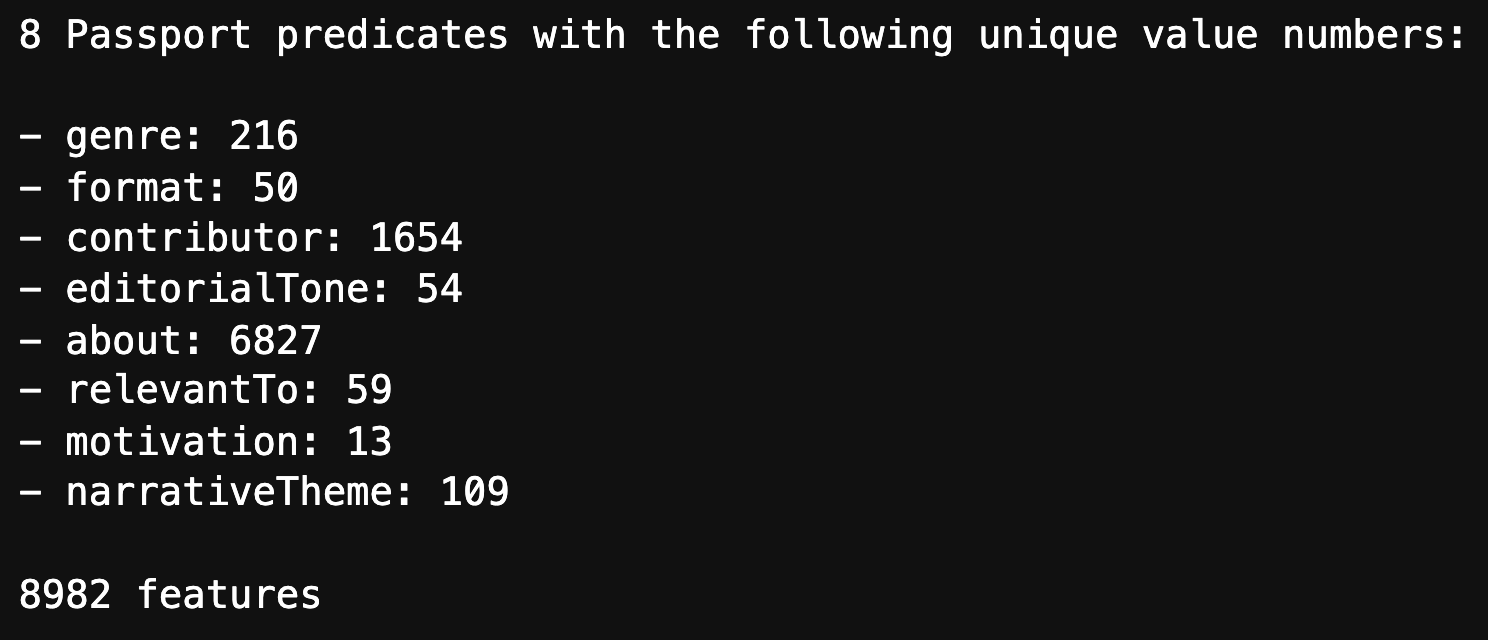
\includegraphics[scale=0.5]{passport_stats}
  \caption{Number of unique value annotations per Passport tag}
  \label{fig:passport_stats}
\end{figure}

\begin{figure}[H]
  \centering
  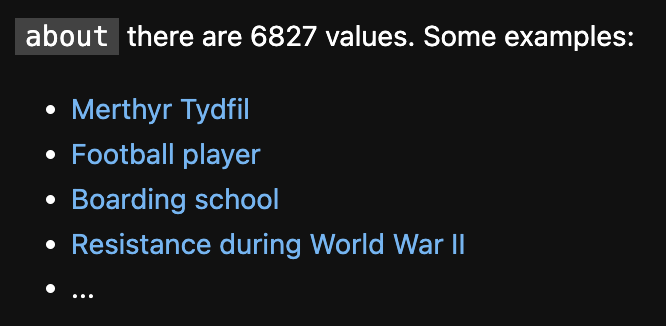
\includegraphics[scale=0.8]{tag_about}
  \caption{The "about" tag}
  \label{fig:tag_about}
\end{figure}

\begin{figure}[H]
  \centering
  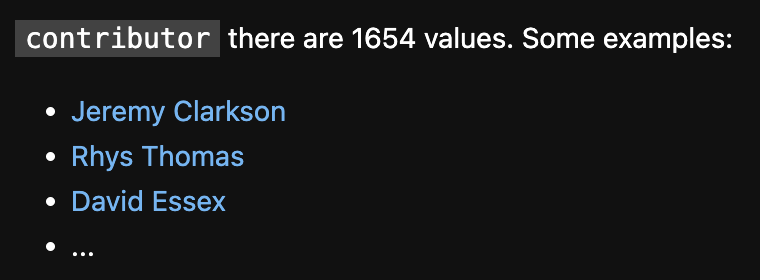
\includegraphics[scale=0.8]{tag_contributor}
  \caption{The "contributor" tag}
  \label{fig:tag_contributor}
\end{figure}

\begin{figure}[H]
  \centering
  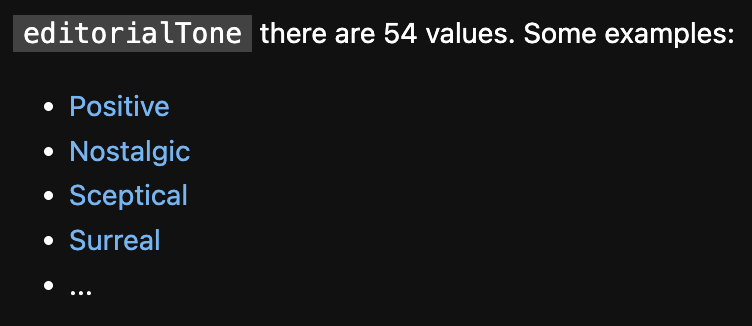
\includegraphics[scale=0.8]{tag_editorialTone}
  \caption{The "editorialTone" tag}
  \label{fig:tag_editorialTone}
\end{figure}

\begin{figure}[H]
  \centering
  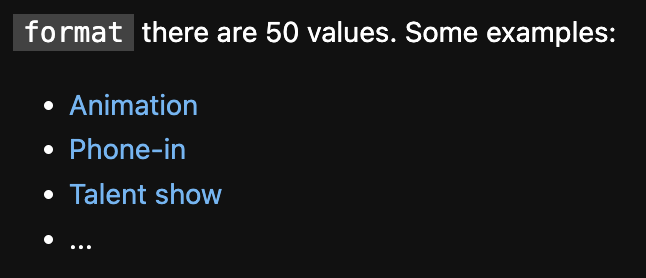
\includegraphics[scale=0.8]{tag_format}
  \caption{The "format" tag}
  \label{fig:tag_format}
\end{figure}

\begin{figure}[H]
  \centering
  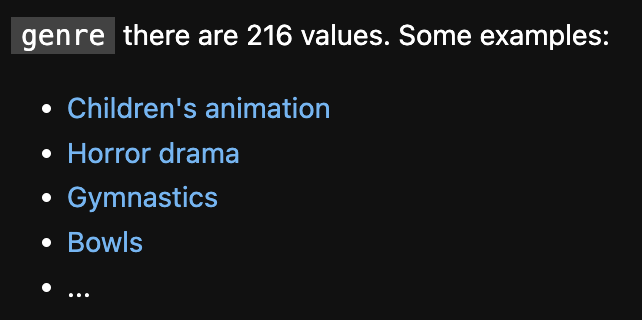
\includegraphics[scale=0.8]{tag_genre}
  \caption{The "genre" tag}
  \label{fig:tag_genre}
\end{figure}

\begin{figure}[H]
  \centering
  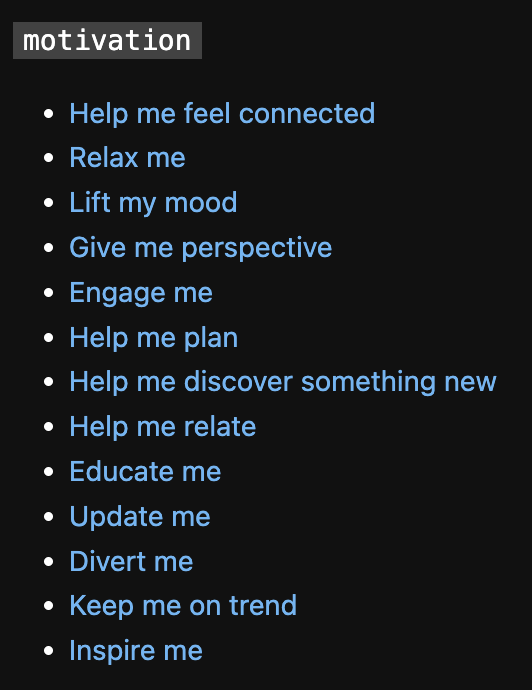
\includegraphics[scale=0.8]{tag_motivation}
  \caption{The "motivation" tag}
  \label{fig:tag_motivation}
\end{figure}

\begin{figure}[H]
  \centering
  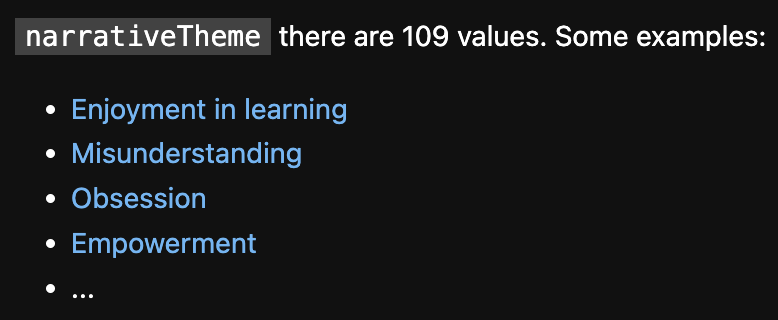
\includegraphics[scale=0.8]{tag_narrativeTheme}
  \caption{The "narrativeTheme" tag}
  \label{fig:tag_narrativeTheme}
\end{figure}

\begin{figure}[H]
  \centering
  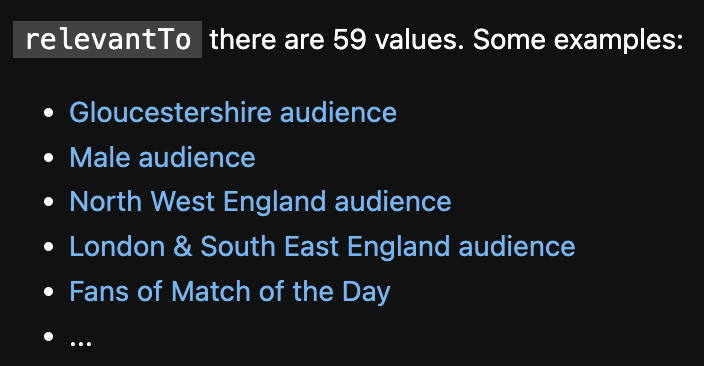
\includegraphics[scale=0.8]{tag_relevantTo}
  \caption{The "relevantTo" tag}
  \label{fig:tag_relevantTo}
\end{figure}

\subsubsection{Catalogue analysis}

The following line plots visualise the daily time-series statistics of the BBC iPlayer catalogue used for training.
New programmes are added to the catalogue, and unavailable ones are removed hourly.
These updates change the size and tag composition of the catalogue and need to be monitored for data drift detection,
retraining the model when big spikes occur.

\begin{figure}[H]
  \centering
  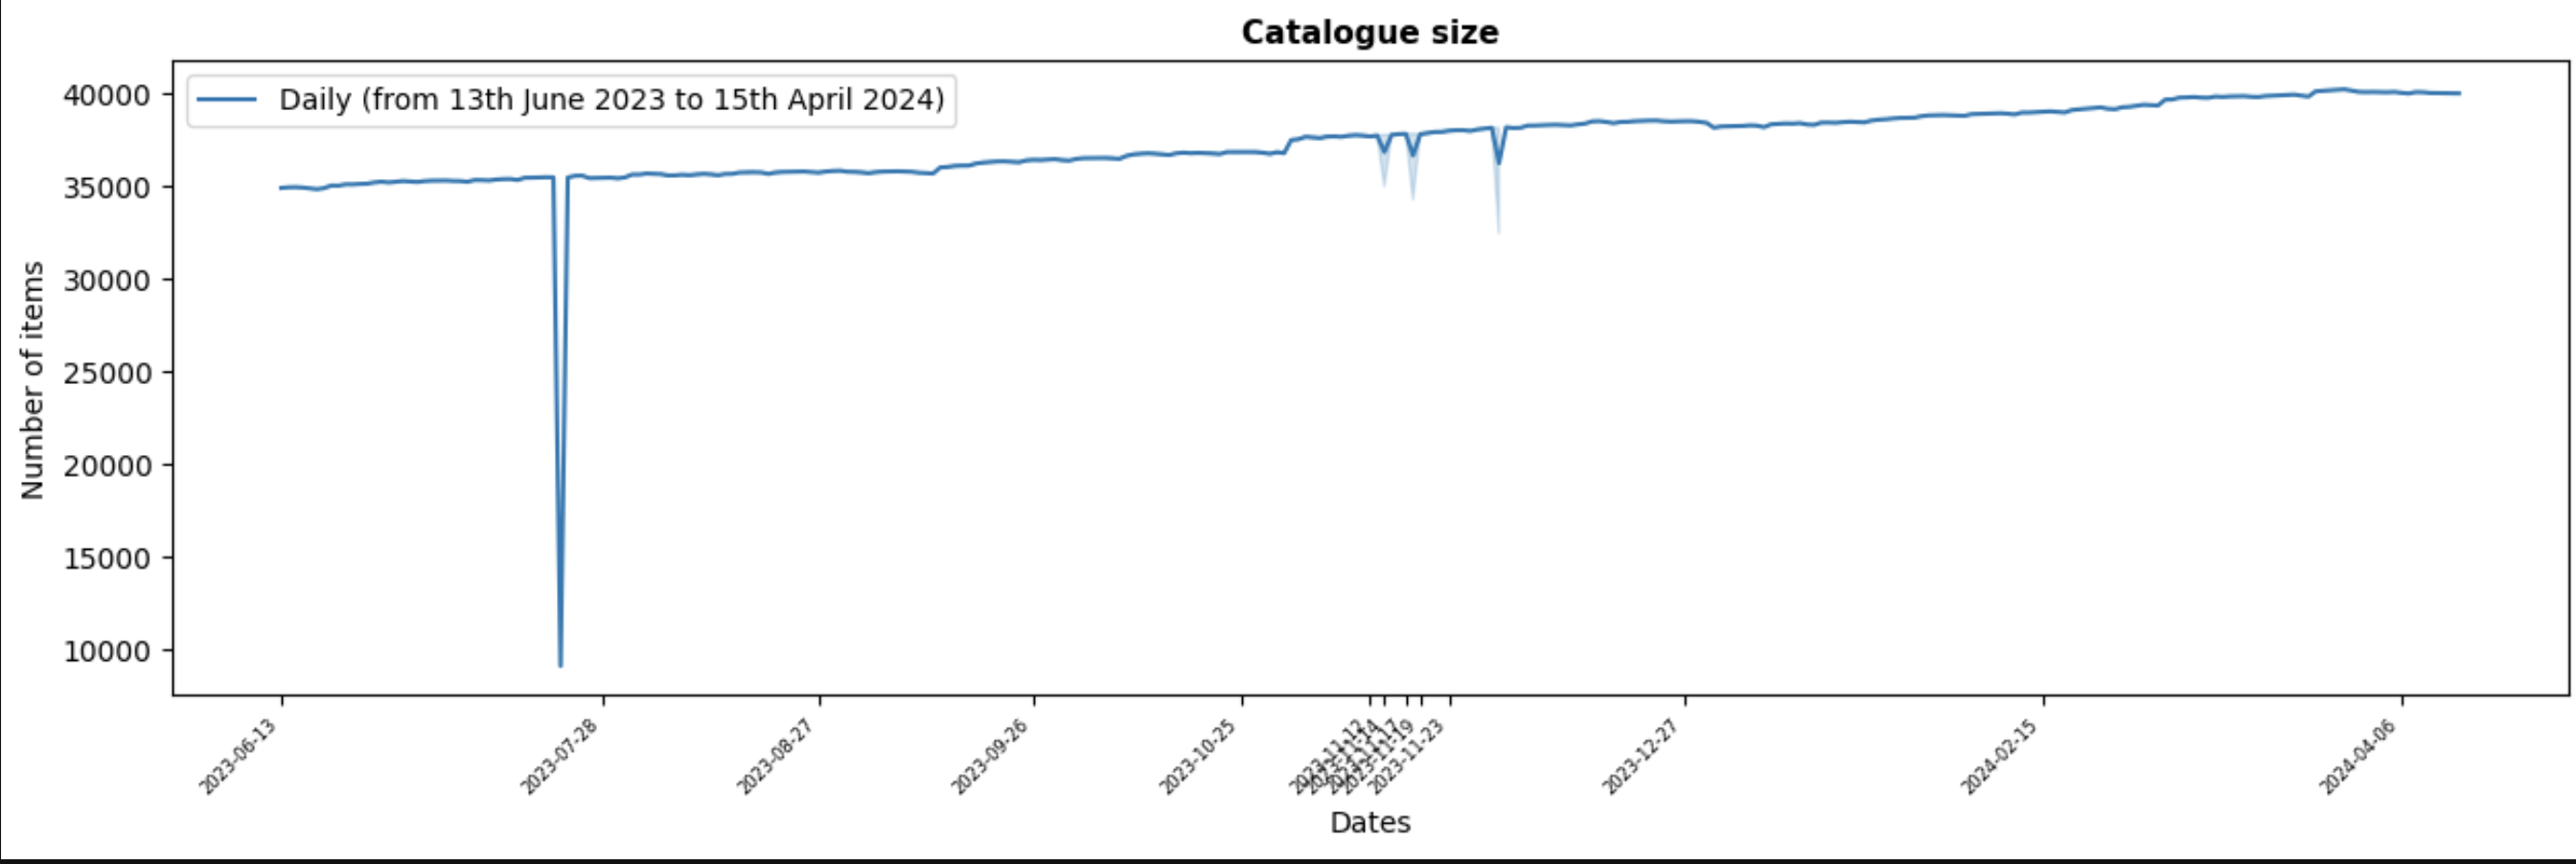
\includegraphics[scale=0.3]{catalogue_size}
  \caption{Daily catalogue size}
  \label{fig:catalogue_size}
\end{figure}

\begin{figure}[H]
  \centering
  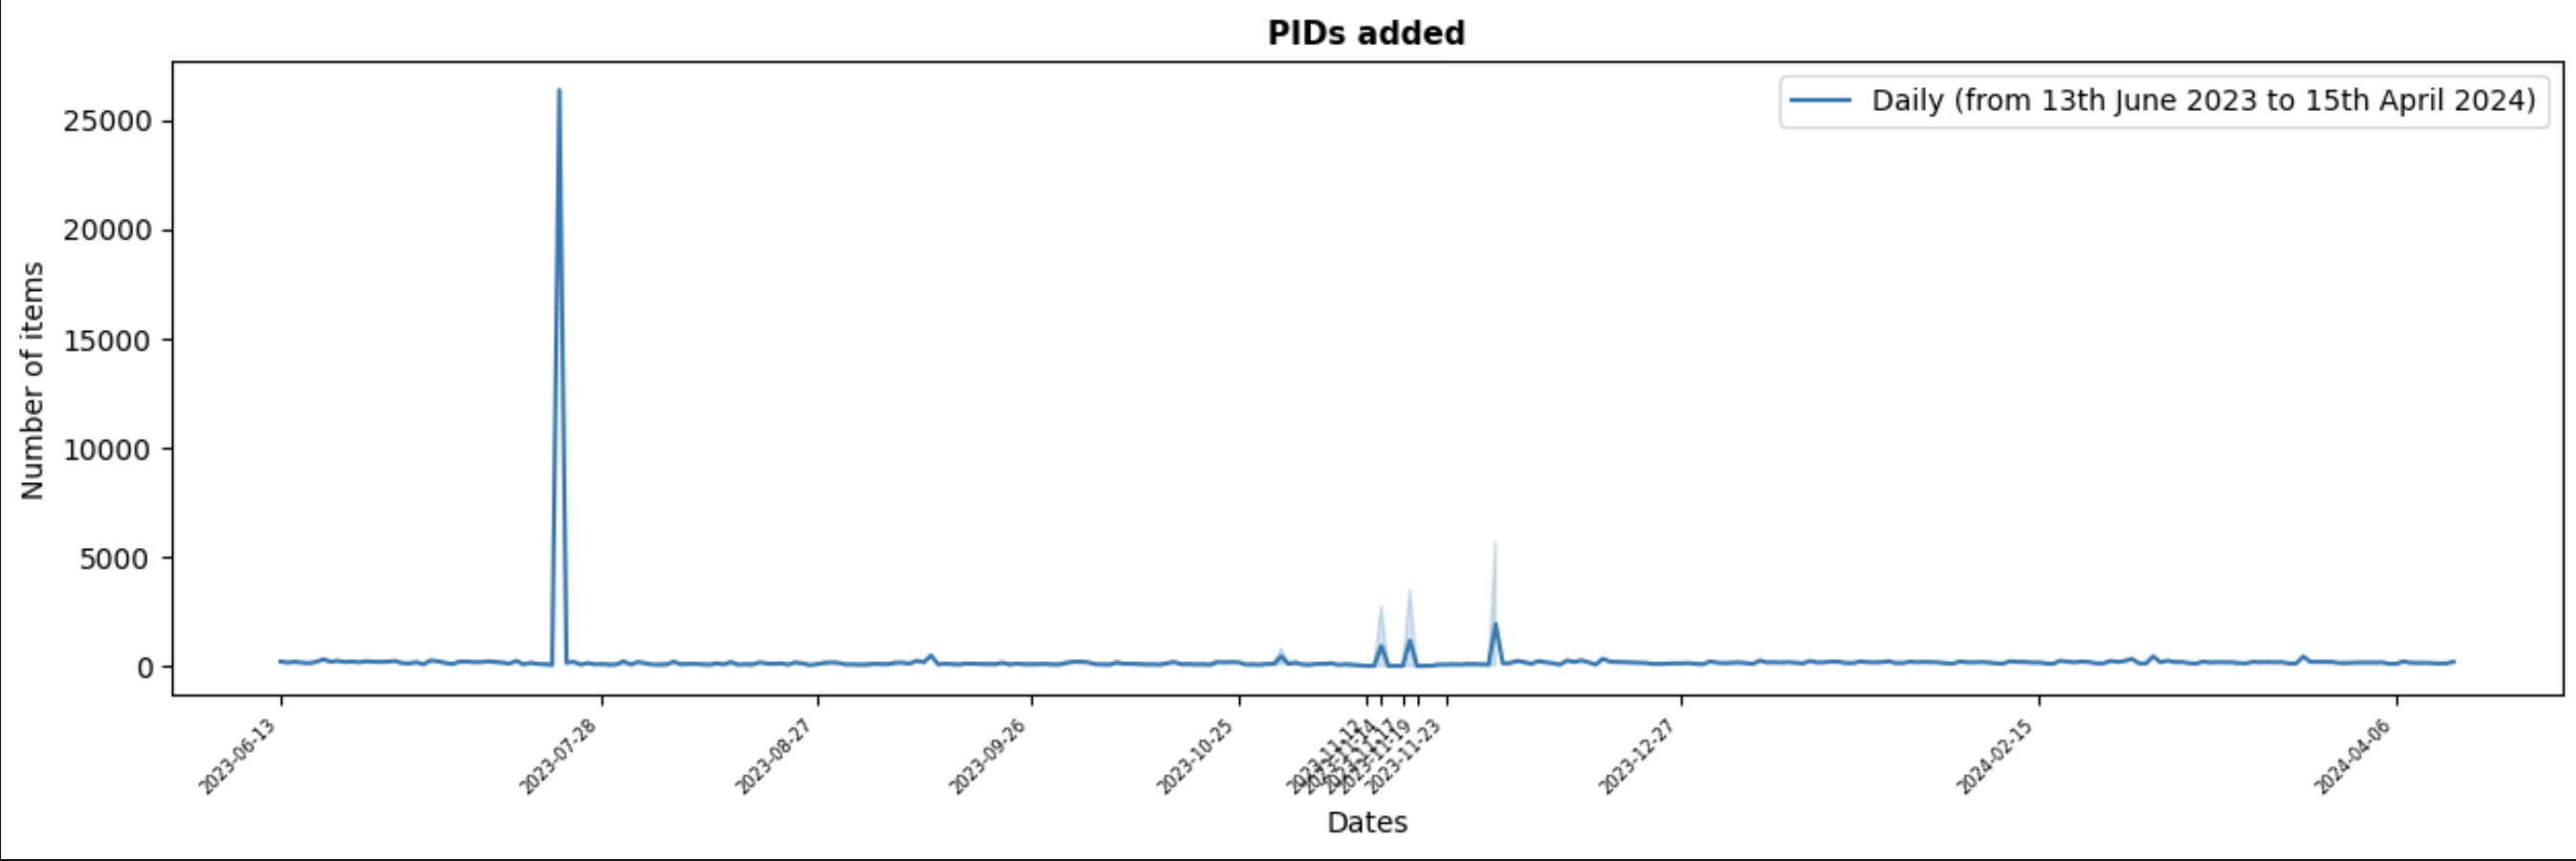
\includegraphics[scale=0.3]{catalogue_pids_added}
  \caption{Number of PIDs added daily}
  \label{fig:catalogue_pids_added}
\end{figure}

\begin{figure}[H]
  \centering
  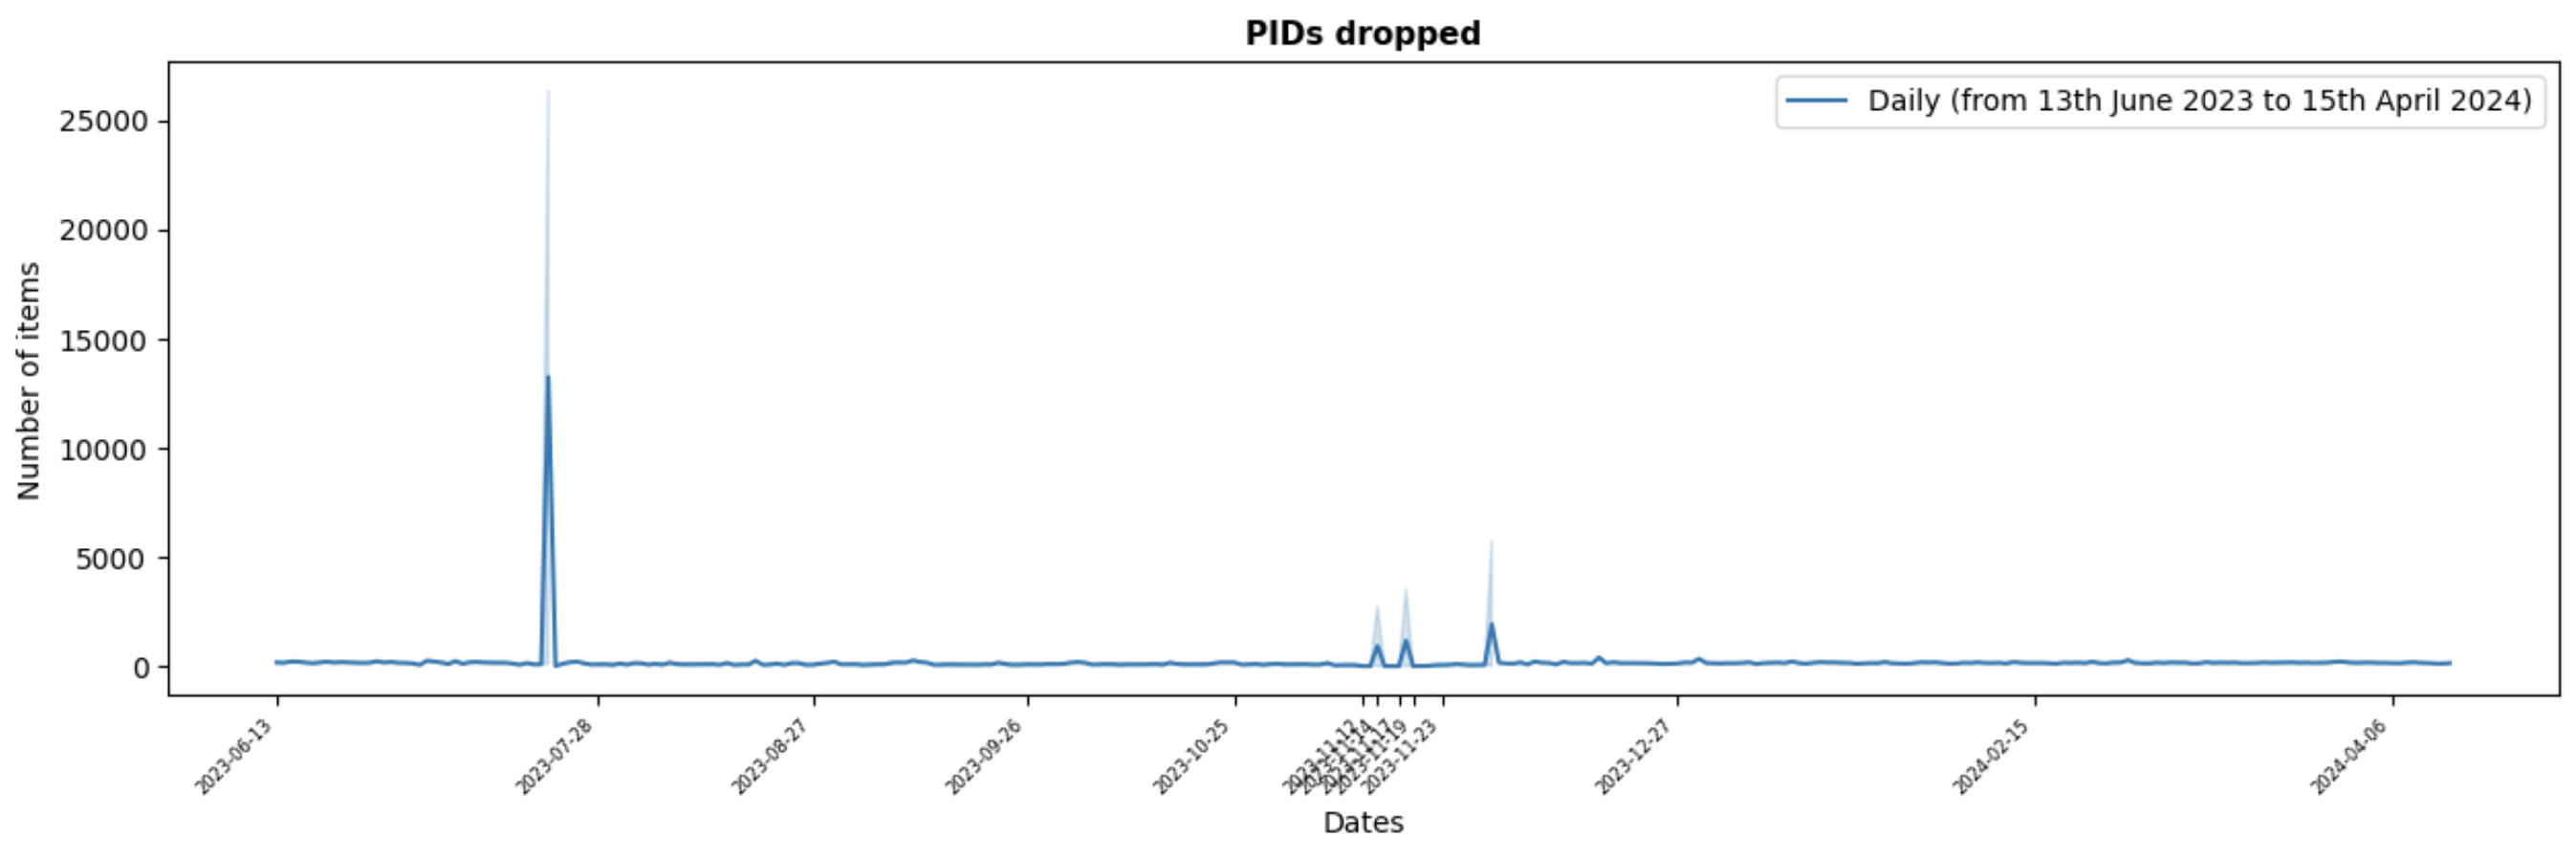
\includegraphics[scale=0.3]{catalogue_pids_dropped}
  \caption{Number of PIDs dropped daily}
  \label{fig:catalogue_pids_dropped}
\end{figure}

\begin{figure}[H]
  \centering
  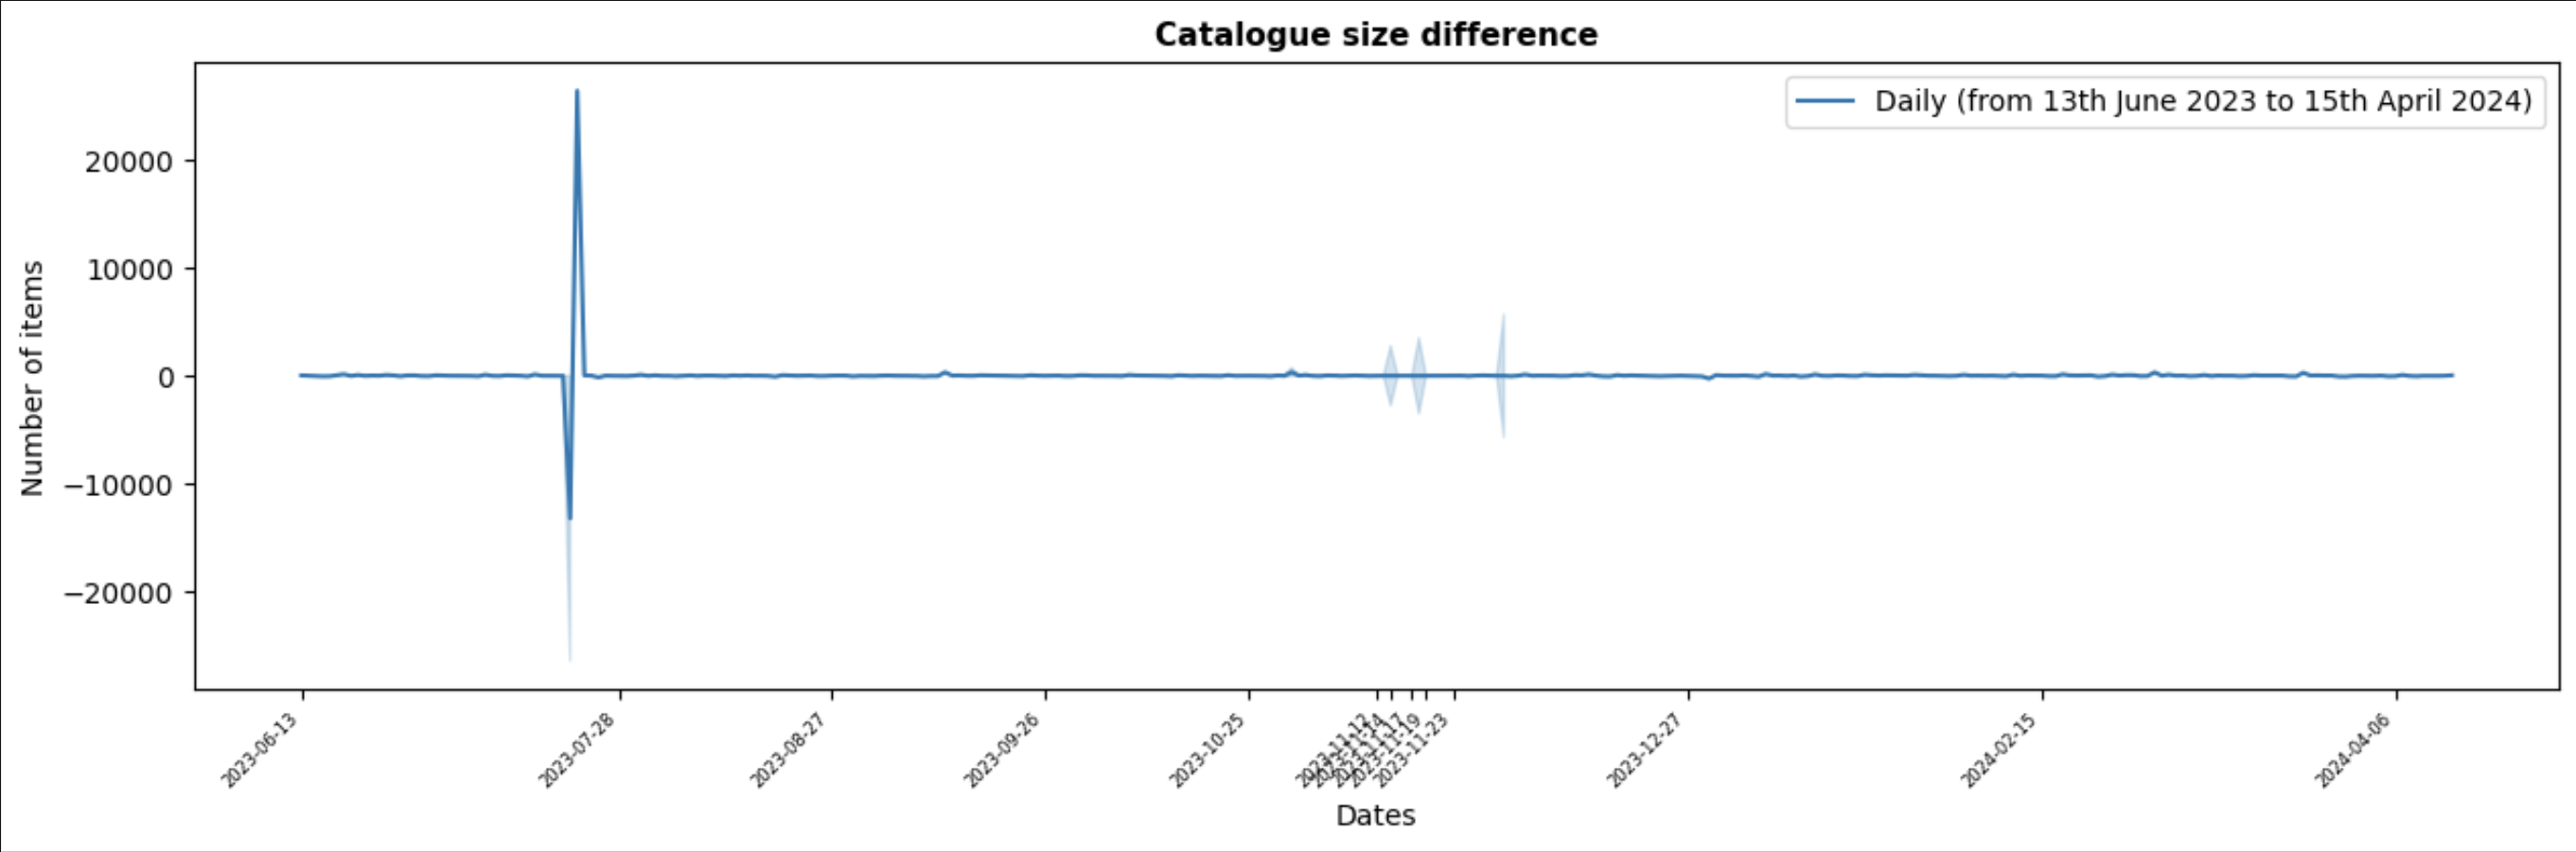
\includegraphics[scale=0.3]{catalogue_size_difference}
  \caption{Daily catalogue size difference}
  \label{fig:catalogue_size_diff}
\end{figure}

\begin{figure}[H]
  \centering
  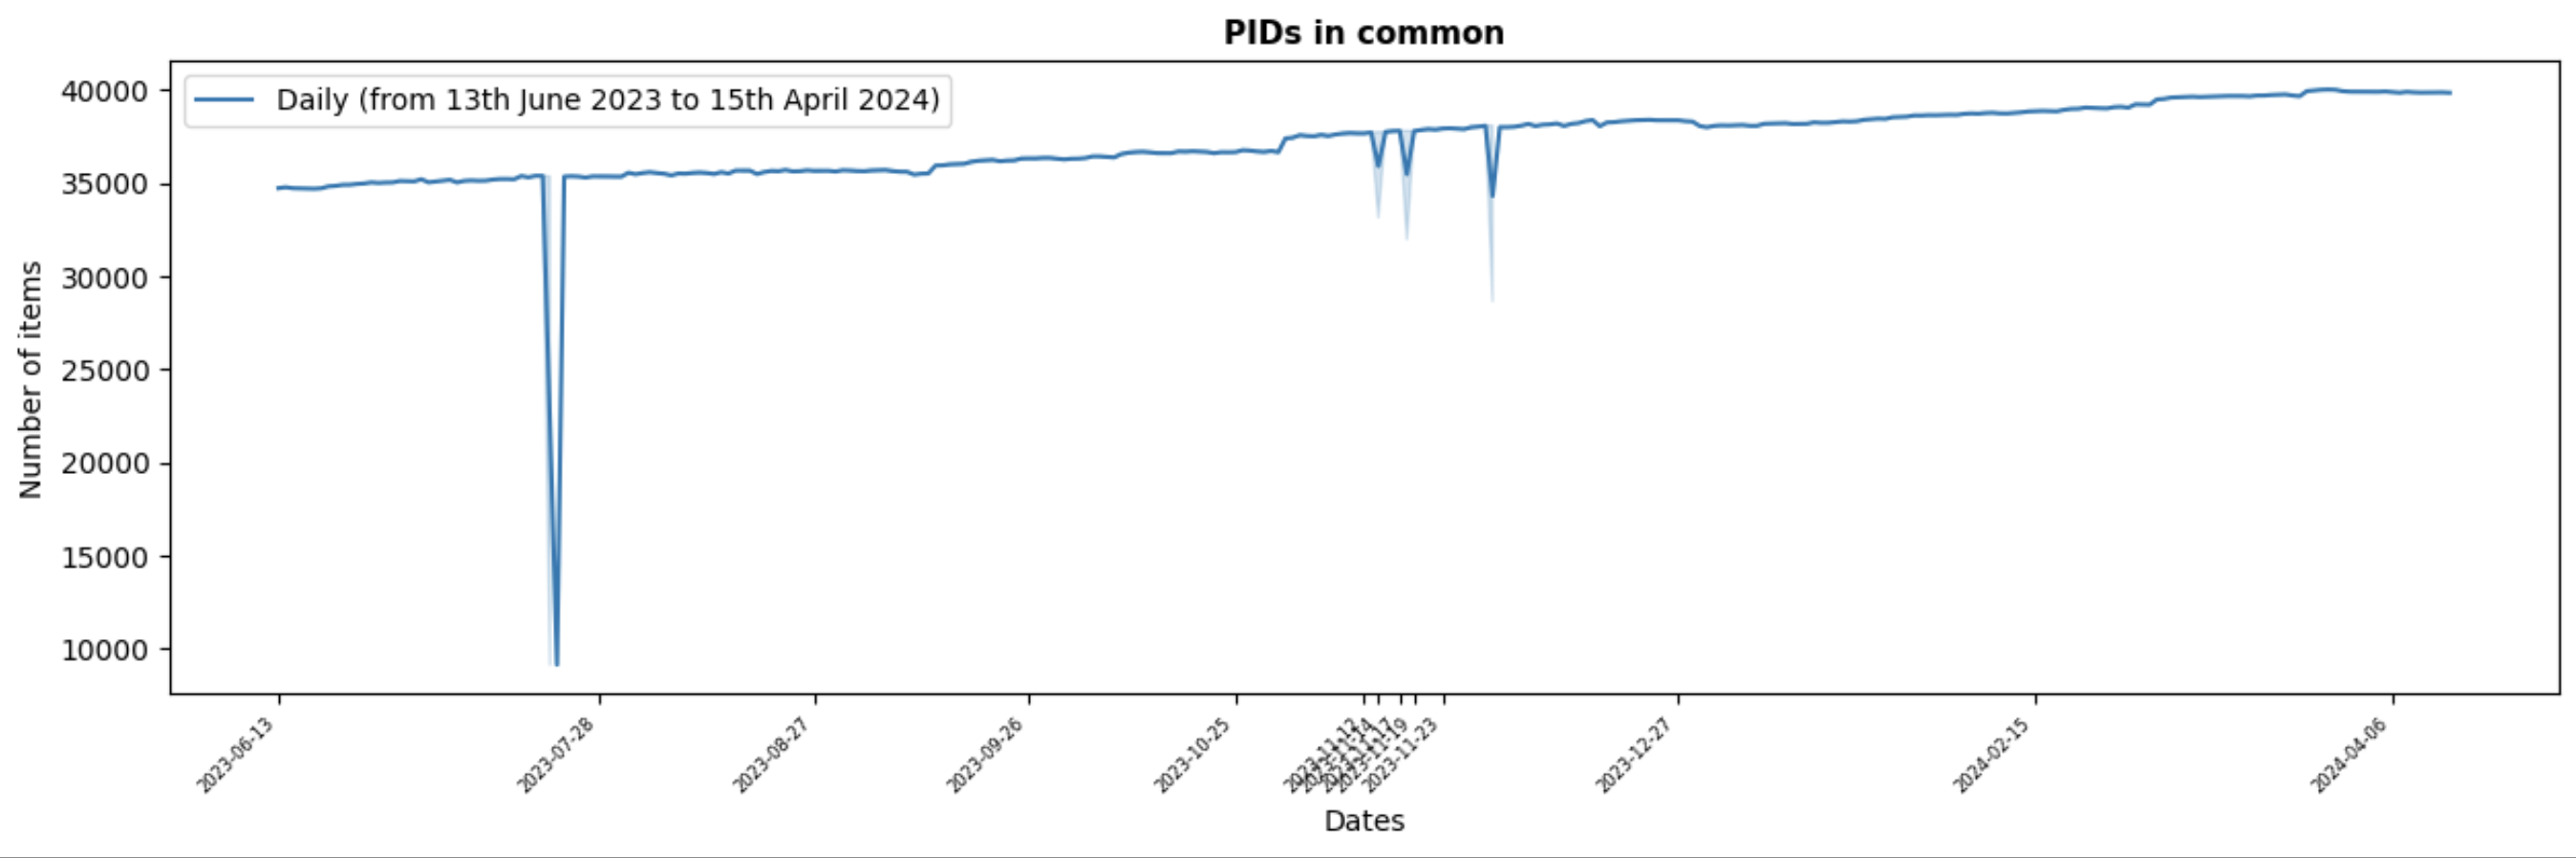
\includegraphics[scale=0.3]{catalogue_pids_common}
  \caption{Number of PIDs in common daily}
  \label{fig:catalogue_pids_common}
\end{figure}

\subsubsection{Programme structure and data distribution}

The \verb|18.19%| of programmes have a \textit{brand-episode} structure.
An example is the ``Christmas Celebration'' show, presented by Sally Magnusson.

\begin{figure}[H]
  \centering
  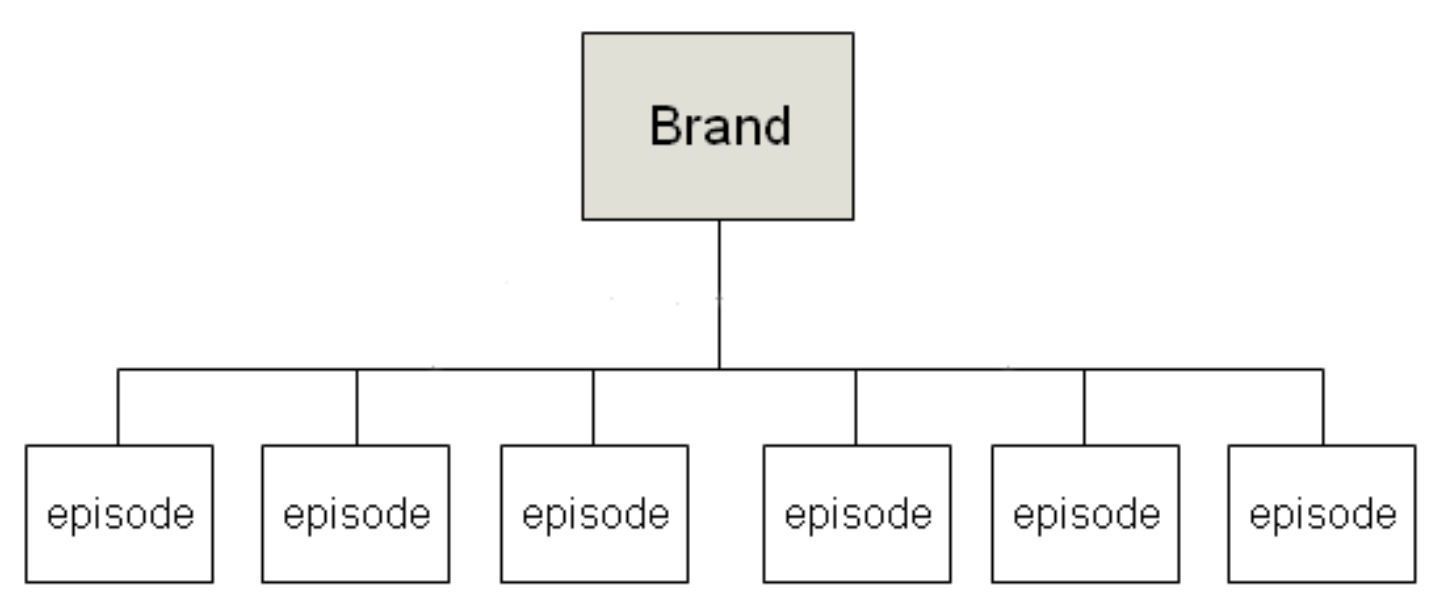
\includegraphics[scale=0.5]{pips_brand}
  \caption{PIP Brand-Episode hierarchy}
  \label{fig:pips_brand}
\end{figure}

The \verb|3.25%| of programmes have a Series-Episode structure.
An example is the four-part series ``Inside Obama's White House''.

\begin{figure}[H]
  \centering
  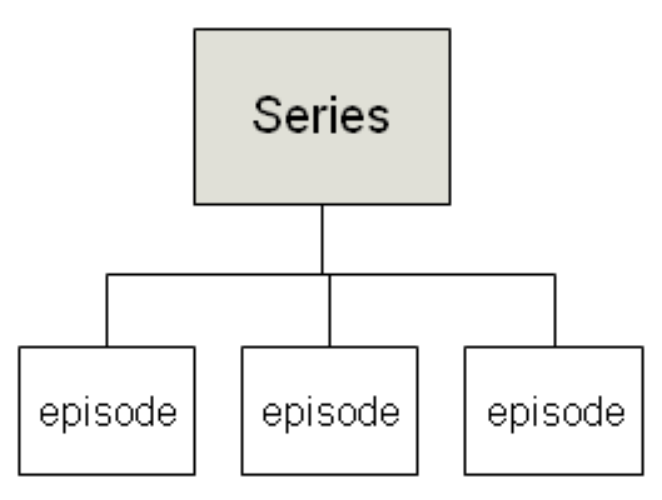
\includegraphics[scale=0.5]{pips_series}
  \caption{PIP Series-Episode hierarchy}
  \label{fig:pips_series}
\end{figure}

The \verb|75.12%| of programmes have a Brand-Series-Episode structure.
An example is the animated adventure comedy series ``Go Jetters''.

\begin{figure}[H]
  \centering
  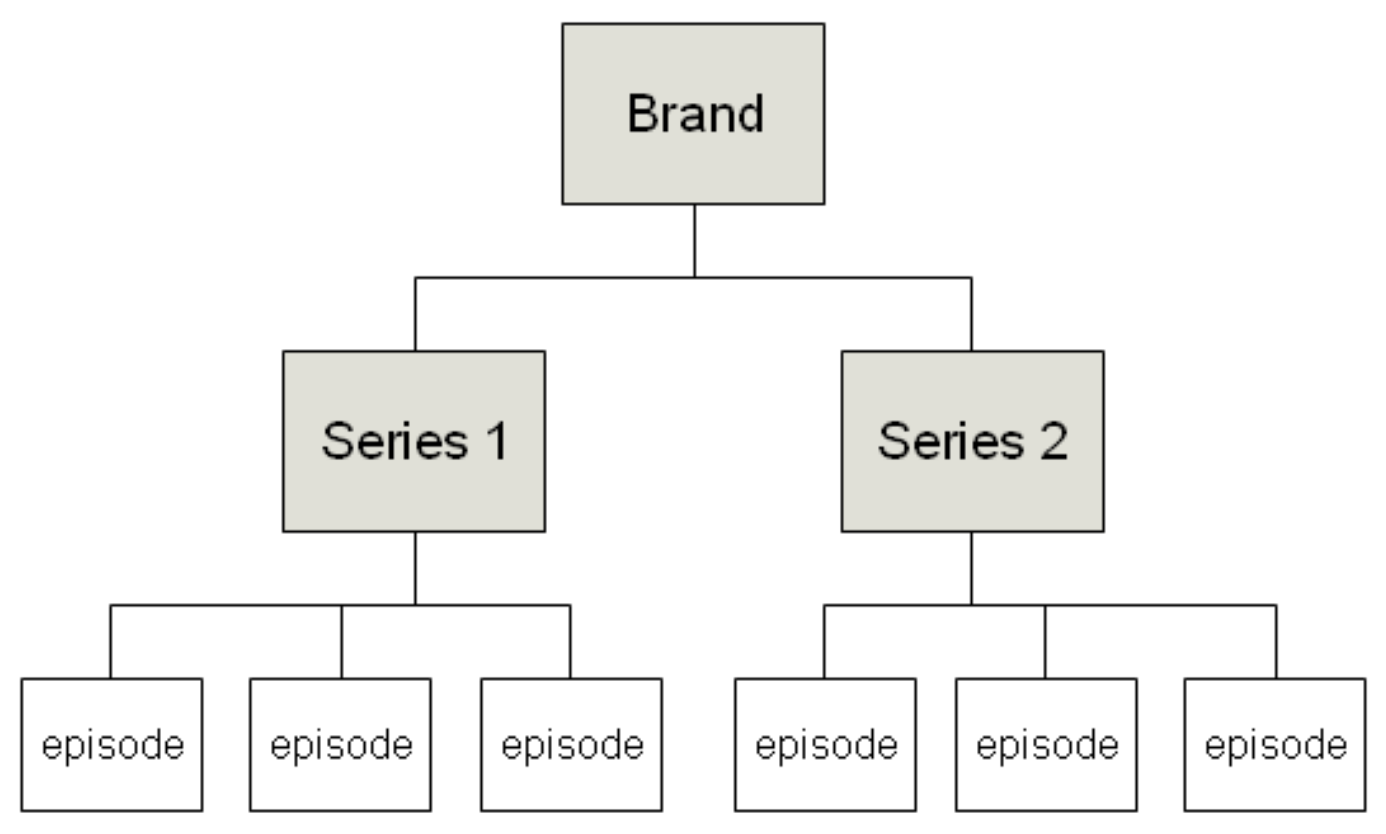
\includegraphics[scale=0.5]{pips_brand_series}
  \caption{PIP Brand-Series-Episode hierarchy}
  \label{fig:pips_brand_series}
\end{figure}

The remaining \verb|3.44%| of programmes are \textit{episode} only.
An example is the comedy documentary ``The Kemps: All Gold'' about the Spandau Ballet brother's lives.

\begin{figure}[H]
  \centering
  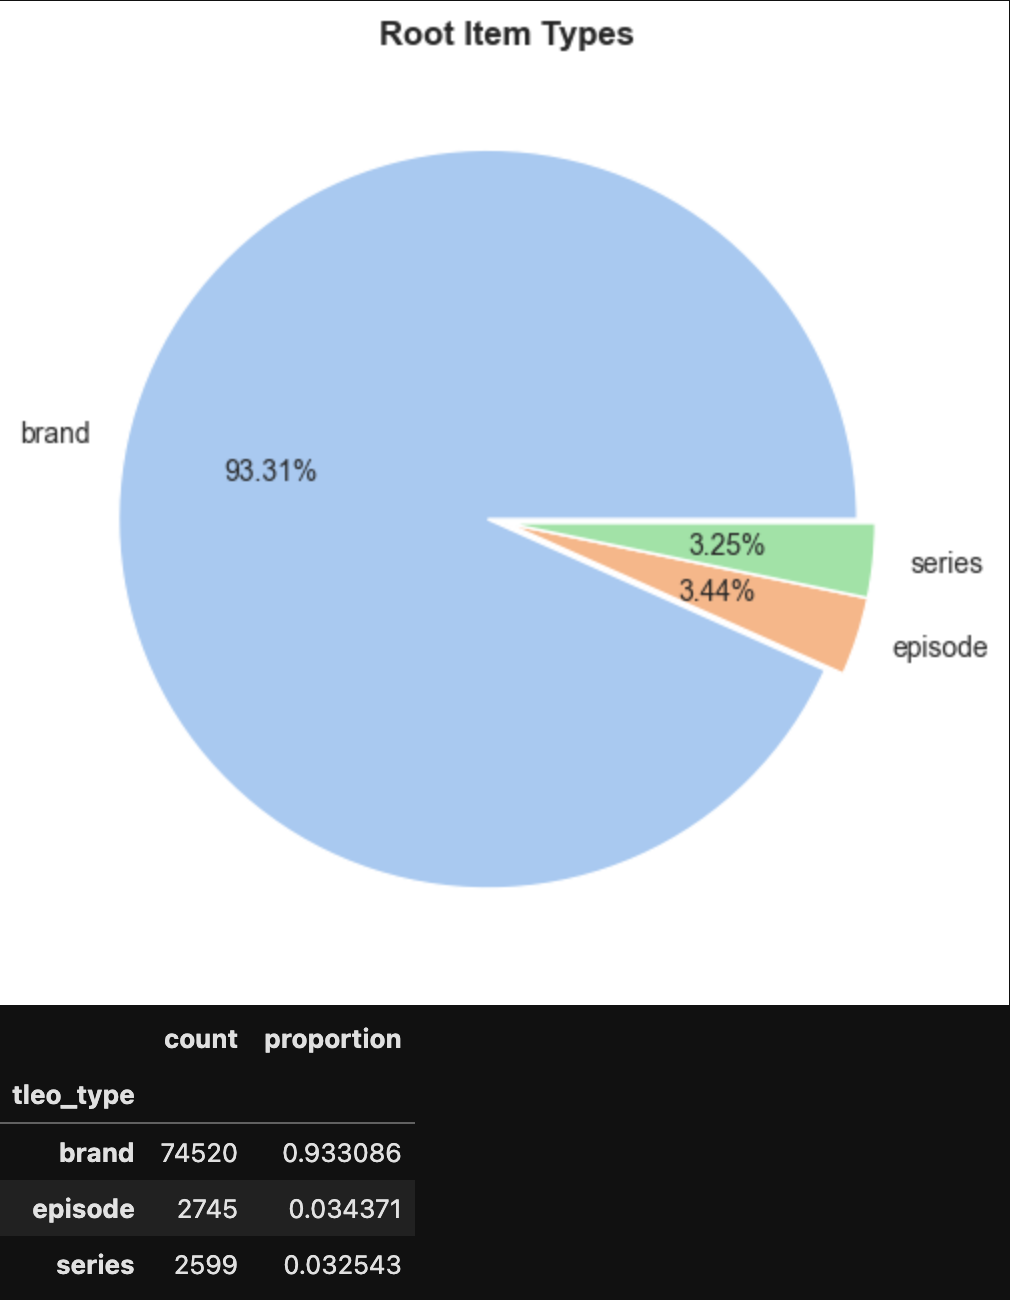
\includegraphics[scale=0.5]{programmes_root_item_types}
  \caption{Root item types distribution}
  \label{fig:programmes_root_item_types}
\end{figure}

\begin{figure}[H]
  \centering
  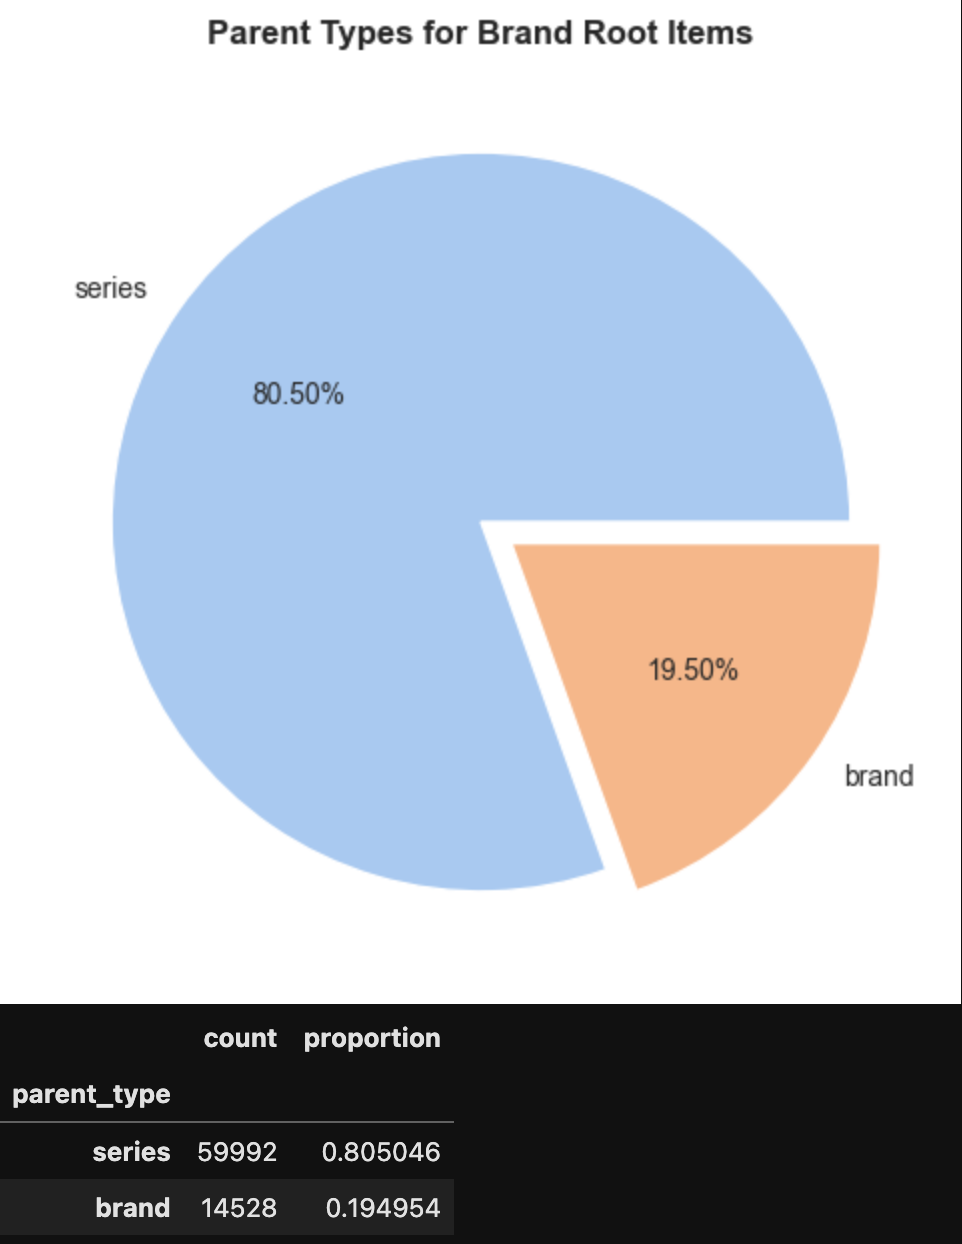
\includegraphics[scale=0.5]{programmes_parent_type.png}
  \caption{Parent types when the root item is a Brand}
  \label{fig:programmes_parent_type}
\end{figure}

\subsubsection{Recommendations}

This is an example of quality testing using the visualisation tool, comparing the generated recommendations
with the ones live on BBC iPlayer.

\begin{figure}[H]
  \centering
  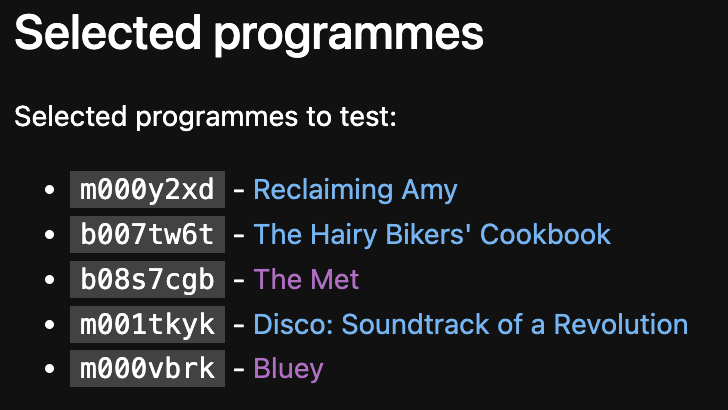
\includegraphics[scale=0.5]{selected_programmes}
  \caption{List of example programmes used for testing}
  \label{fig:selected_programmes}
\end{figure}

Figure \ref{fig:bluey} shows the programme page for "Bluey" and the "More Like This" section on iPlayer,
where 12 similar programmes are recommended.

\begin{figure}[H]
  \centering
  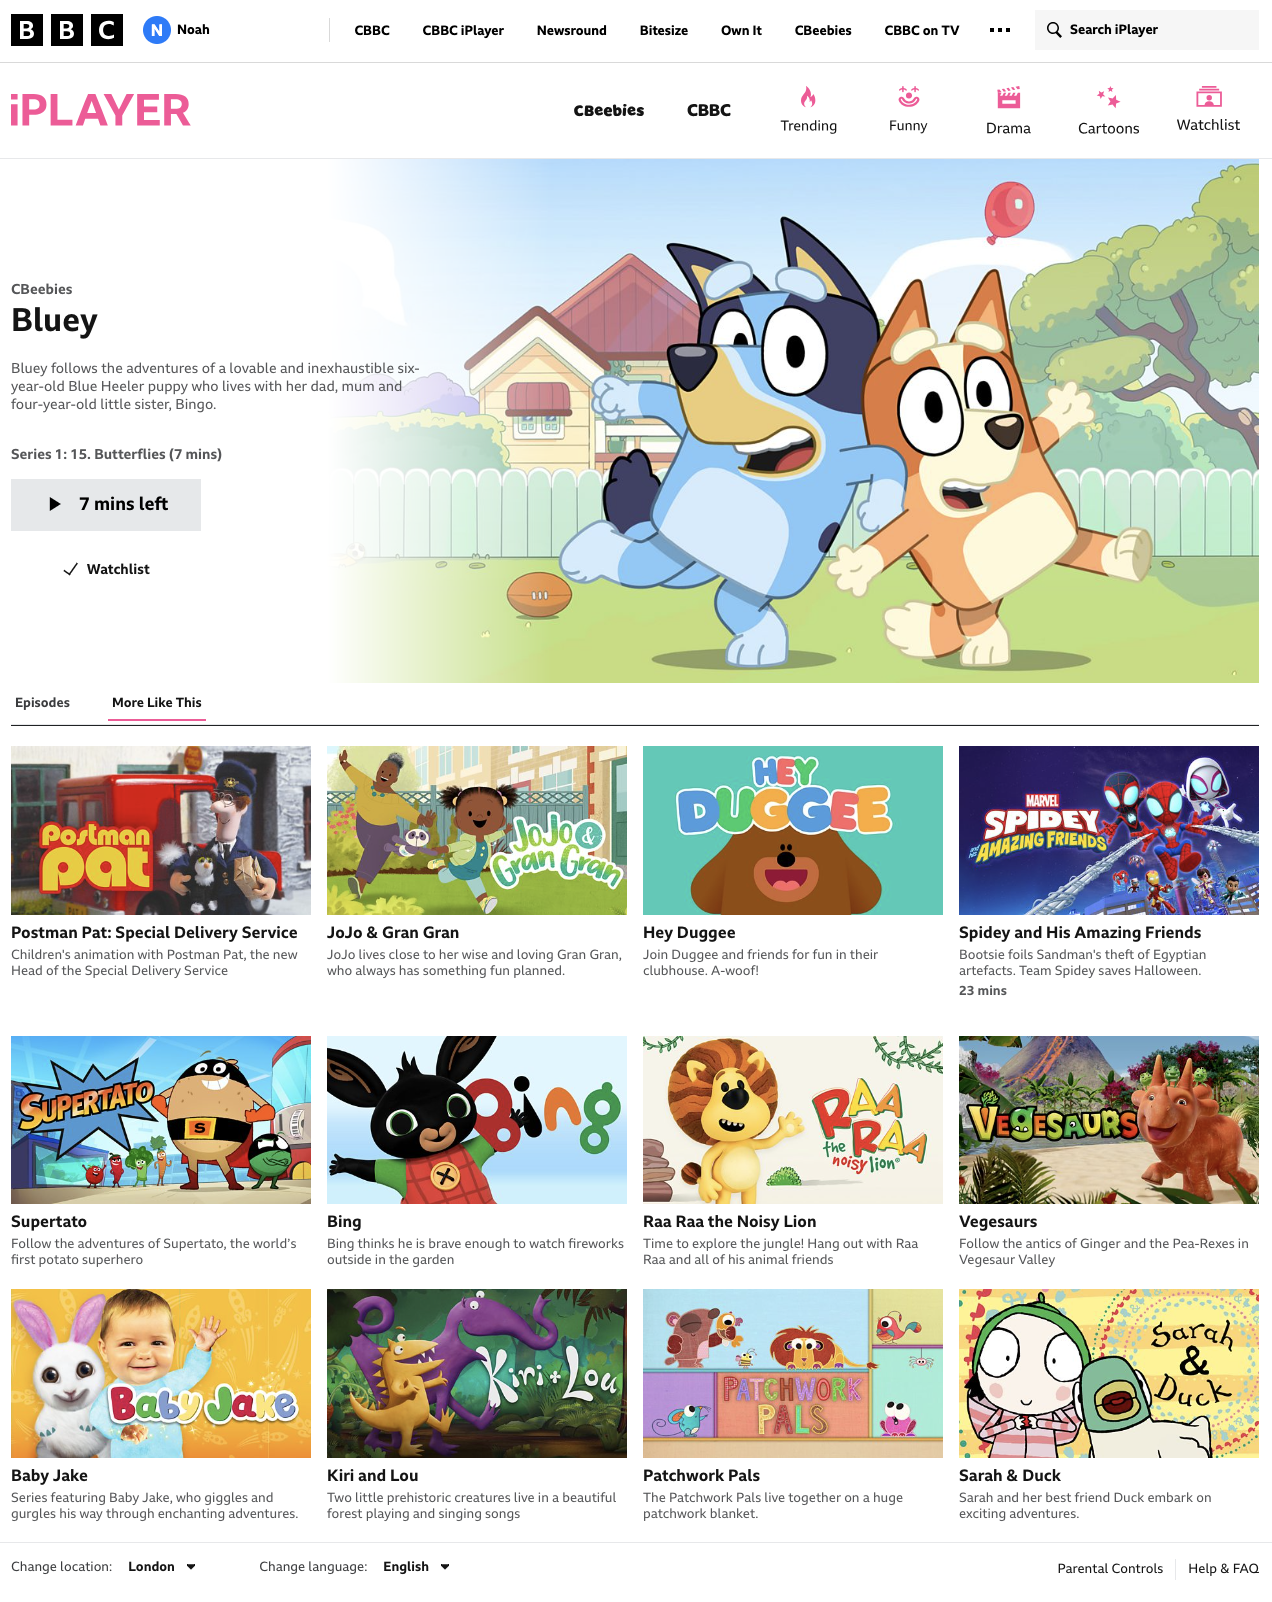
\includegraphics[scale=0.5]{bluey}
  \caption{The ``More Like This'' section on BBC iPlayer}
  \label{fig:bluey}
\end{figure}

Figure \ref{fig:recommendations:0} shows the seed programme for the top-12 content similarity recommendations.

\begin{figure}[H]
  \centering
  
\includegraphics[scale=0.5]{recommendations/0}
  \caption{``Bluey'' (the seed programme)}
  \label{fig:recommendations:0}
\end{figure}

The following figures show the recommendations generated by the pipeline in descending order of similarity score (the percentage in the parenthesis).

\begin{figure}[H]
  \centering
  
\includegraphics[scale=0.5]{recommendations/1}
  \caption{``Patchwork Pals'' (96.017\%) }
  \label{fig:recommendations:1}
\end{figure}

\begin{figure}[H]
  \centering
  
\includegraphics[scale=0.5]{recommendations/2}
  \caption{``Timmy Time'' (94.737\%)}
  \label{fig:recommendations:2}
\end{figure}

\begin{figure}[H]
  \centering
  
\includegraphics[scale=0.5]{recommendations/3}
  \caption{``Fireman Sam'' (94.199\%)}
  \label{fig:recommendations:3}
\end{figure}

\begin{figure}[H]
  \centering
  
\includegraphics[scale=0.5]{recommendations/4}
  \caption{``Arthur'' (94.061\%)}
  \label{fig:recommendations:4}
\end{figure}

\begin{figure}[H]
  \centering
  
\includegraphics[scale=0.5]{recommendations/5}
  \caption{``Postman Pat: Special Delivery Service'' (93.940\%)}
  \label{fig:recommendations:5}
\end{figure}

\begin{figure}[H]
  \centering
  
\includegraphics[scale=0.5]{recommendations/6}
  \caption{``Tish Tash'' (93.734\%)}
  \label{fig:recommendations:6}
\end{figure}

\begin{figure}[H]
  \centering
  
\includegraphics[scale=0.5]{recommendations/7}
  \caption{``Octonauts'' (93.241\%)}
  \label{fig:recommendations:7}
\end{figure}

\begin{figure}[H]
  \centering
  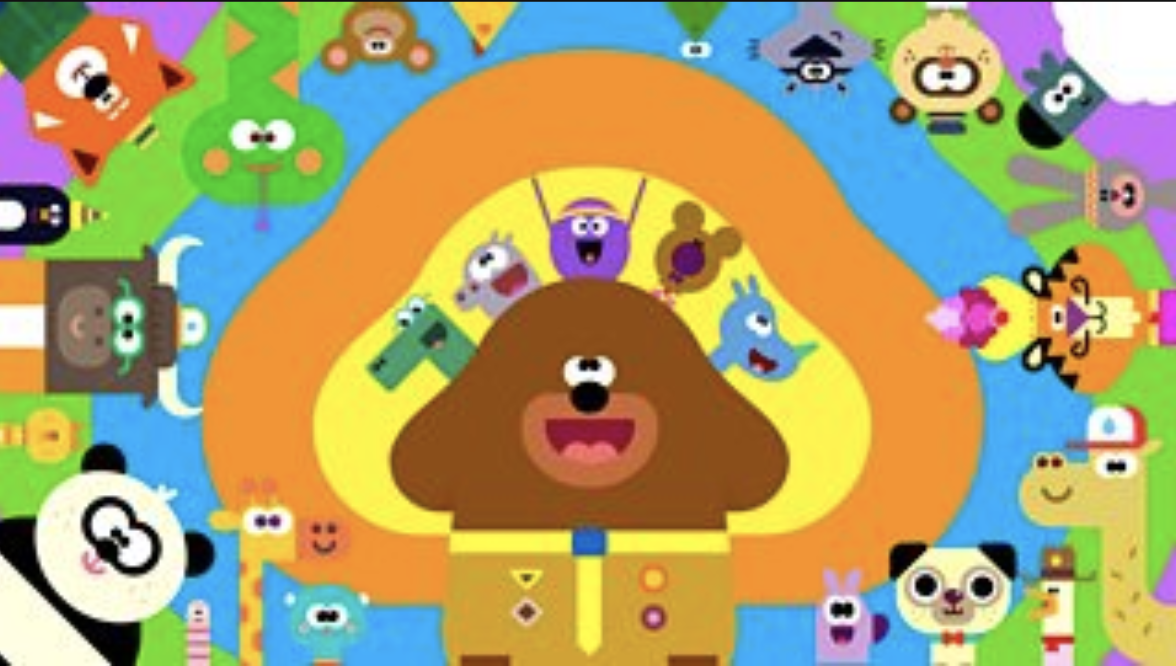
\includegraphics[scale=0.5]{recommendations/8}
  \caption{``Hey Duggee'' (93.237\%)}
  \label{fig:recommendations:8}
\end{figure}

\begin{figure}[H]
  \centering
  
\includegraphics[scale=0.5]{recommendations/9}
  \caption{``Bob the Builder'' (93.012\%)}
  \label{fig:recommendations:9}
\end{figure}

\begin{figure}[H]
  \centering
  
\includegraphics[scale=0.5]{recommendations/10}
  \caption{``Tee and Mo'' (92.761\%)}
  \label{fig:recommendations:10}
\end{figure}

\begin{figure}[H]
  \centering
  
\includegraphics[scale=0.5]{recommendations/11}
  \caption{``Raa Raa the Noisy Lion'' (92.487\%)}
  \label{fig:recommendations:11}
\end{figure}

\begin{figure}[H]
  \centering
  
\includegraphics[scale=0.5]{recommendations/12}
  \caption{``Mr Bear's Christmas'' (92.303\%)}
  \label{fig:recommendations:12}
\end{figure}

\newpage

% This is highly recommended
% The level of detail needed is section headings and page numbers illustrating where the criteria have been met
\subsection{Mapping of the project report to the pass criteria}

\begin{figure}[H]
  \centering
  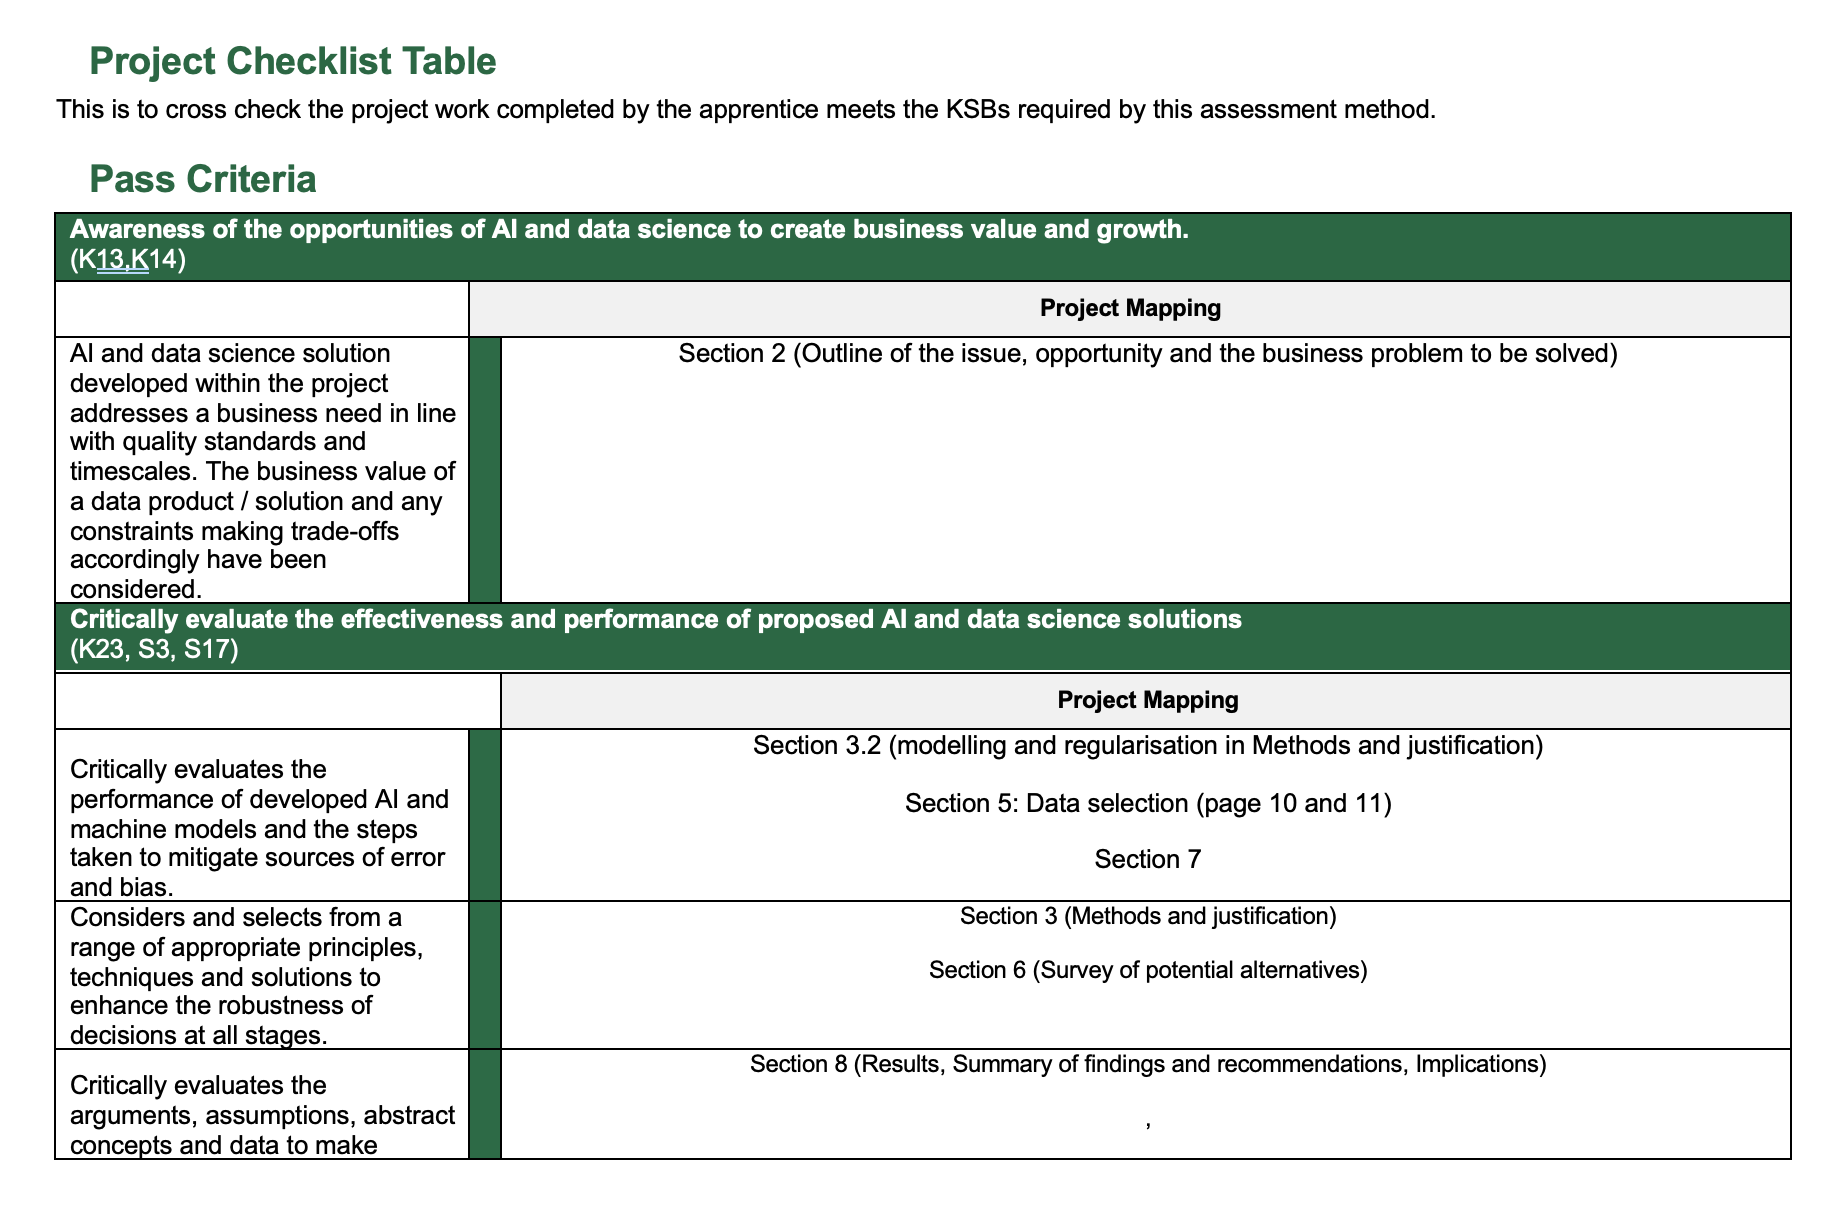
\includegraphics[scale=0.5]{mapping/0}
  \caption{Mapping: page 1}
  \label{fig:mapping:0}
\end{figure}

\begin{figure}[H]
  \centering
  
\includegraphics[scale=0.5]{mapping/1}
  \caption{Mapping: page 2}
  \label{fig:mapping:1}
\end{figure}

\begin{figure}[H]
  \centering
  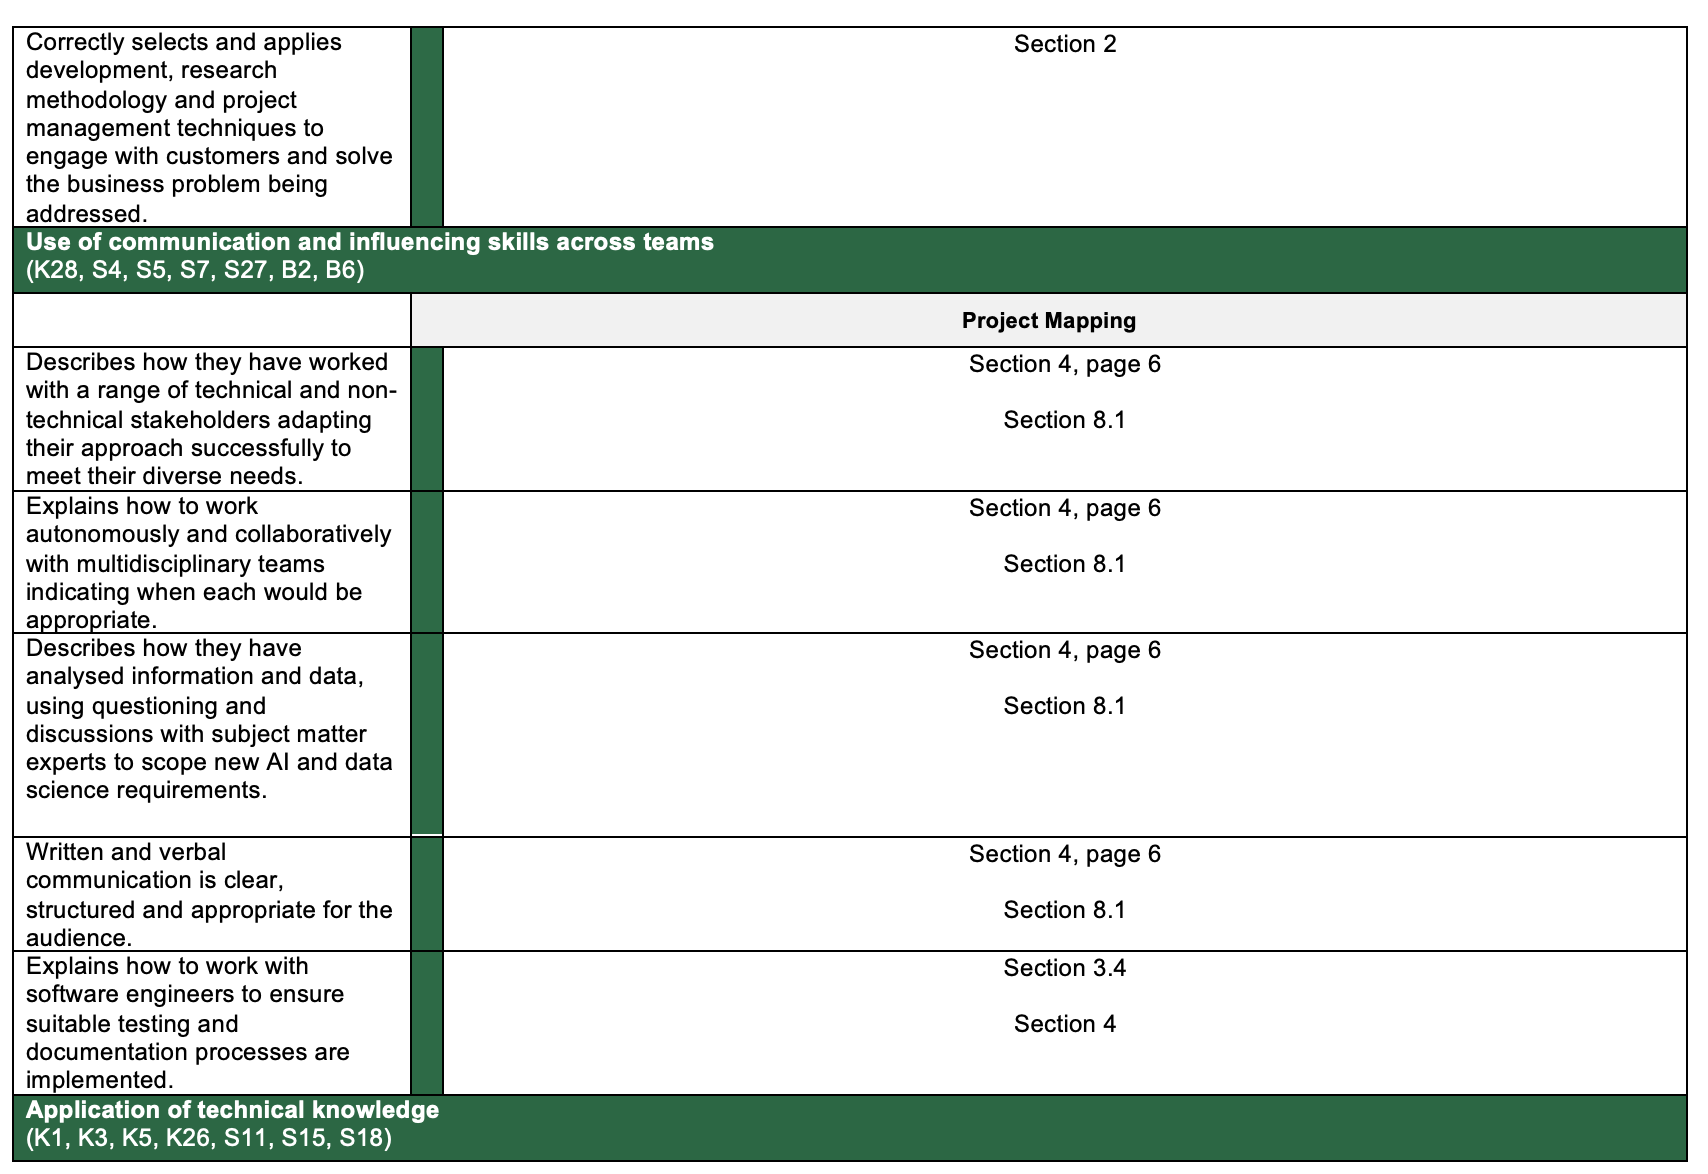
\includegraphics[scale=0.5]{mapping/2}
  \caption{Mapping: page 3}
  \label{fig:mapping:2}
\end{figure}

\begin{figure}[H]
  \centering
  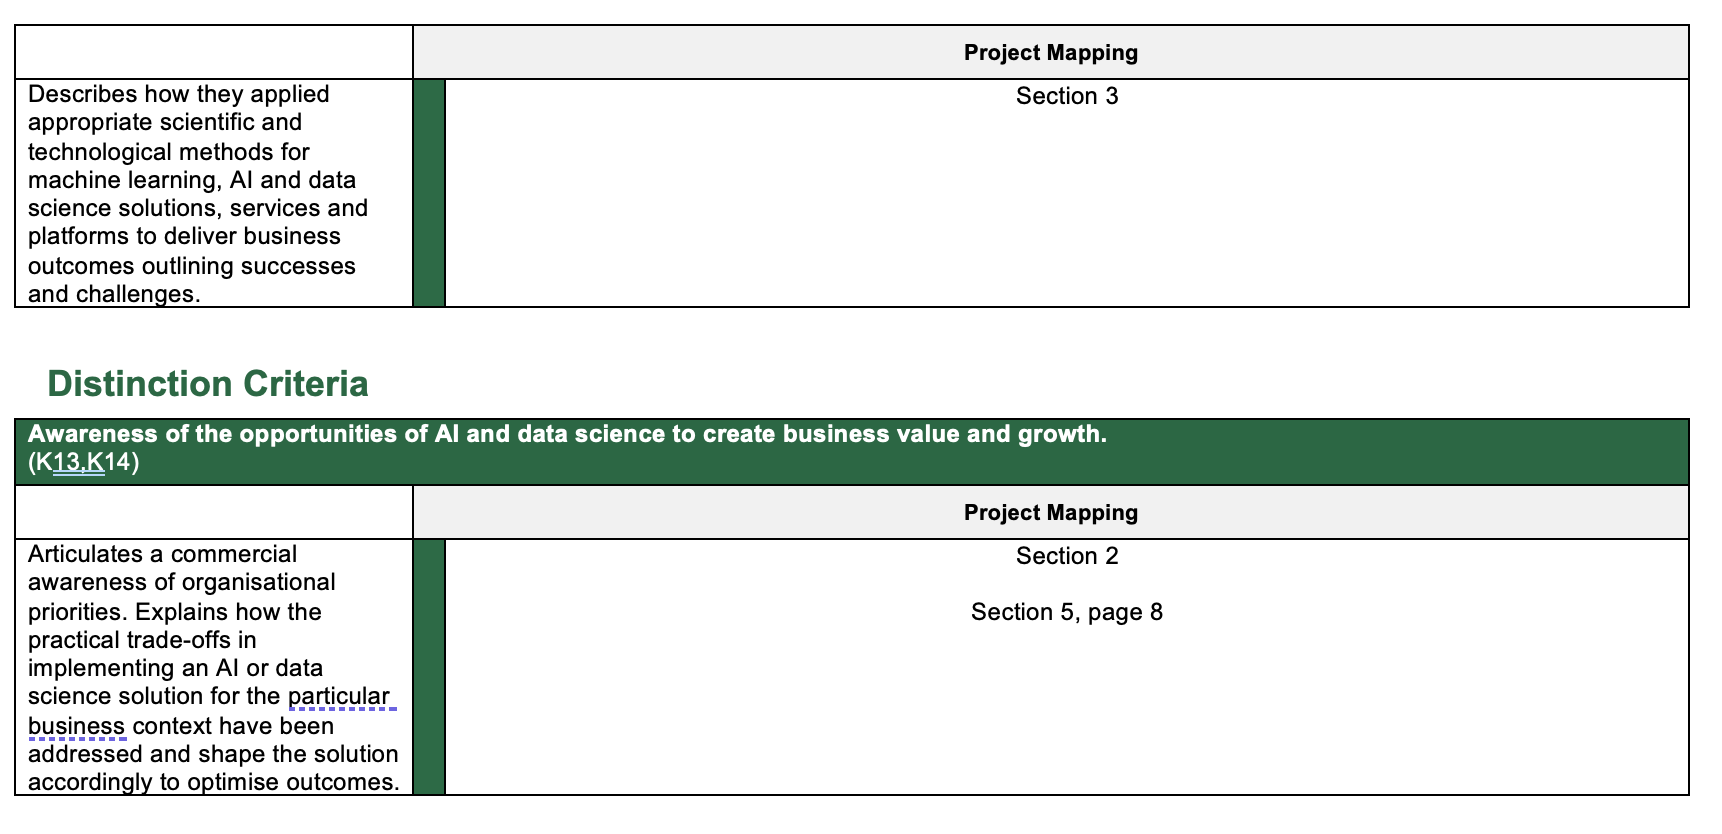
\includegraphics[scale=0.5]{mapping/3}
  \caption{Mapping: page 4}
  \label{fig:mapping:3}
\end{figure}

\begin{figure}[H]
  \centering
  
\includegraphics[scale=0.5]{mapping/4}
  \caption{Mapping: page 5}
  \label{fig:mapping:4}
\end{figure}

\begin{figure}[H]
  \centering
  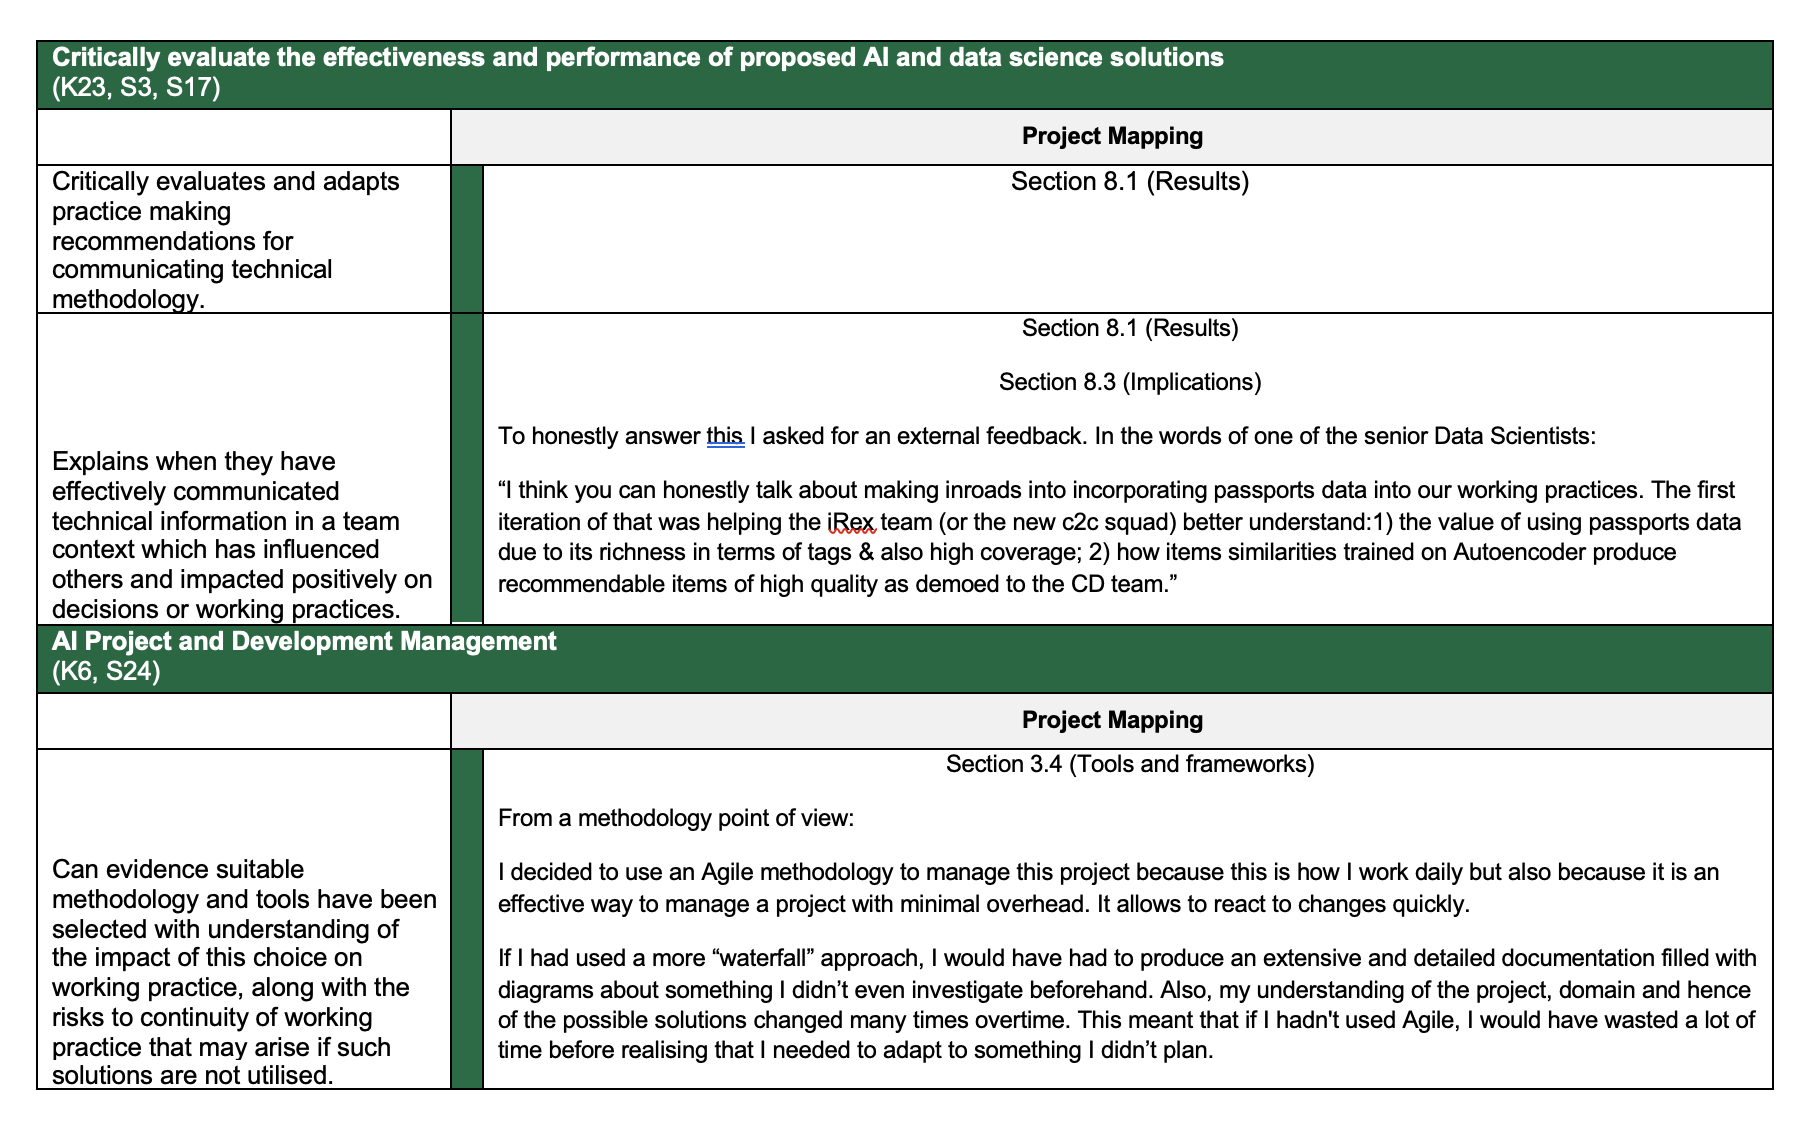
\includegraphics[scale=0.5]{mapping/5}
  \caption{Mapping: page 6}
  \label{fig:mapping:5}
\end{figure}


\bibliography{refs}
\bibliographystyle{plain}

\end{document}
